\documentclass[10pt,a4paper]{article}
\usepackage[margin=2.3cm]{geometry}
\usepackage[T1]{fontenc}
\usepackage{lmodern}
\usepackage{amsmath,amssymb,mathtools}
\usepackage{graphicx,float,booktabs,xcolor}
\usepackage[hidelinks,colorlinks=true,linkcolor=blue!50!black,urlcolor=blue!50!black]{hyperref}
\setlength{\parindent}{0pt}\setlength{\parskip}{4pt}
\setcounter{secnumdepth}{2}

% ---------- notation ----------
\newcommand{\R}{\mathbb{R}}
\newcommand{\vv}[1]{\mathbf{#1}}
\newcommand{\abs}[1]{\left|#1\right|}
\newcommand{\norm}[1]{\left\lVert#1\right\rVert}
\newcommand{\clamp}{\operatorname{clamp}}
\newcommand{\sdbox}{\operatorname{sdBox}}
\newcommand{\sortd}{\operatorname{sort}_{\downarrow}}
\newcommand{\fract}{\operatorname{fract}}
\newcommand{\atantwo}{\operatorname{atan2}}
\newcommand{\Rot}{\mathsf{R}}
\newcommand{\DE}{\mathrm{DE}}
\newcommand{\ex}{\vv{e}_x}\newcommand{\ey}{\vv{e}_y}\newcommand{\ez}{\vv{e}_z}
\newcommand{\sfold}{\operatorname{sphereFold}}
\newcommand{\bfold}{\operatorname{boxFold}}

\title{\textbf{Fractal Video: the equations}\\[2pt]\large Every distance estimator in \texttt{vfx-apps/fractal-video/js/formulas.js}}
\author{Brokild Apps}
\date{\today}

\begin{document}
\maketitle
\tableofcontents

\section{How to read this document}

The program is a GPU ray marcher. It does \emph{not} draw fractals by plotting points: for every pixel it
marches a ray through space, and at each step asks a function $\DE(\vv p)$ ``how far is the nearest surface from here?''.
Every fractal in the program is therefore \emph{one formula}: a \textbf{distance estimator} (DE) written in GLSL.
This document translates all 34 of them into mathematics. For each one you get the iteration, the distance estimate, what
the parameters do (with the app's default values), and a picture.

\paragraph{About the pictures.} The renders are made by a small stand-alone ray marcher that loads the \emph{same GLSL distance
functions} from \texttt{formulas.js} with each formula's default parameters, default iteration count and default camera. The
lighting and colouring are a simple stand-in (sun + soft shadow + orbit-trap colour), \emph{not} the app's full look pipeline
(palettes, AO, glow, tone-mapping), so colours will differ from what you see in the program. The shapes are exact.

\subsection{The march}
For a ray $\vv r(t)=\vv o+t\,\vv d$ the program steps $t\leftarrow t+\sigma\,\DE(\vv r(t))$ until $\DE<\varepsilon(t)$ (hit) or $t$ is
too large (miss). $\sigma$ is the per-formula \emph{step factor} (below 1 for estimators that overshoot).

\subsection{Global space operations (applied before every formula)}
Before the formula sees a point $\vv p=(x,y,z)$ the program may transform it (the \emph{Space} tab). With twist rate $\tau$, repeat period $\rho$ and bound radius $B$:
\begin{align}
a &= \tau\,y, & \vv q&=\begin{pmatrix}\cos a & \sin a\\ -\sin a&\cos a\end{pmatrix}\!\begin{pmatrix}x\\z\end{pmatrix}\quad\text{(twist about the $y$ axis)}\\
\vv q &\leftarrow \vv q-\rho\,\lfloor \vv q/\rho+\tfrac12\rfloor &&\text{(domain repetition, if $\rho>0$)}\\
d_{\text{march}} &= \sigma\cdot\max\!\big(\DE(\vv q),\;\norm{\vv p}-B\big) &&\text{(bounding sphere, if $B>0$)}
\end{align}

\subsection{Common building blocks}
\begin{itemize}
\item \textbf{Rotations.} $\Rot_A,\Rot_B$ are rotation matrices from Euler angles $(\alpha,\beta,\gamma)$ in degrees, applied $x$ then $y$ then $z$: $\Rot=\Rot_z(\gamma)\Rot_y(\beta)\Rot_x(\alpha)$.
Formulas with one rotation use $\Rot_A$; those with two ($\Rot_A$ pre-, $\Rot_B$ post-rotation) say so.
\item \textbf{Scale--offset map.} $S_{s,\vv o}(\vv z)=s\,\vv z-\vv o\,(s-1)$ (scale about the point $\vv o$).
\item \textbf{Sort fold.} $\sortd(\vv z)$ permutes the components so that $z_x\ge z_y\ge z_z$ (three conditional swaps).
\item \textbf{Box distance.} $\sdbox(\vv q,\vv b)=\norm{\max(\abs{\vv q}-\vv b,\,0)}+\min\!\big(\max(q_x,q_y,q_z),\,0\big)$.
\item \textbf{Running derivative.} Folds and scalings are conformal, so a scalar $\mathrm{dr}$ tracks the accumulated stretch and the final distance is divided by it.
\item \textbf{Orbit trap} (for colouring only, never affects shape): $\vv t=\big(\min\abs{z_x},\min\abs{z_y},\min\abs{z_z},\min\norm{\vv z}^2\big)$ over the orbit.
\end{itemize}

Sphere and box folds used by the Mandelbox family:
\begin{align}
\bfold_f(\vv z)&=2\,\clamp(\vv z,-f,f)-\vv z,\\
\sfold_{m,R}(\vv z,\mathrm{dr}):\quad k&=\begin{cases}R^2/m^2& \norm{\vv z}<m\\ R^2/\norm{\vv z}^2& m\le\norm{\vv z}<R\\ 1&\text{otherwise}\end{cases},\quad \vv z\leftarrow k\vv z,\ \ \mathrm{dr}\leftarrow k\,\mathrm{dr}.
\end{align}
And the \emph{bulb power map} (spherical-coordinate $n$th power) used by the Mandelbulb family:
\begin{equation}
\mathcal B_n(\vv z)=r^{n}\big(\sin\theta\cos\phi,\ \sin\theta\sin\phi,\ \cos\theta\big),\quad r=\norm{\vv z},\ \theta=n\arccos\frac{z_z}{r},\ \phi=n\,\atantwo(z_y,z_x).
\end{equation}

% =====================================================================
\section{Escape-time fractals}

\subsection{Mandelbulb}
Iterate with $\vv z_0=\vv p$ and $\vv c=(1-j)\,\vv p+j\,\vv c_J$ ($j$ = \emph{Julia mix}, $\vv c_J$ = Julia constant):
\begin{align}
r&=\norm{\vv z_k},\quad \theta=n\arccos\frac{z_{k,z}}{r}+\theta_0,\quad \phi=n\,\atantwo(z_{k,y},z_{k,x})+\phi_0,\\
\vv z_{k+1}&=r^{n}\big(\sin\theta\cos\phi,\sin\theta\sin\phi,\cos\theta\big)+\vv c,\\
\mathrm{dr}_{k+1}&=n\,r^{\,n-1}\,\mathrm{dr}_k+(1-j),\qquad \mathrm{dr}_0=1.
\end{align}
Stop when $\norm{\vv z}>2$ or after the iteration limit. The distance estimate (Hubbard--Douady potential)
\begin{equation}\DE(\vv p)=\tfrac12\,\frac{r\,\ln r}{\mathrm{dr}}.\end{equation}
$n$ = \emph{Power} (8 is the classic bulb), $\theta_0,\phi_0$ = phase offsets.
\begin{figure}[H]\centering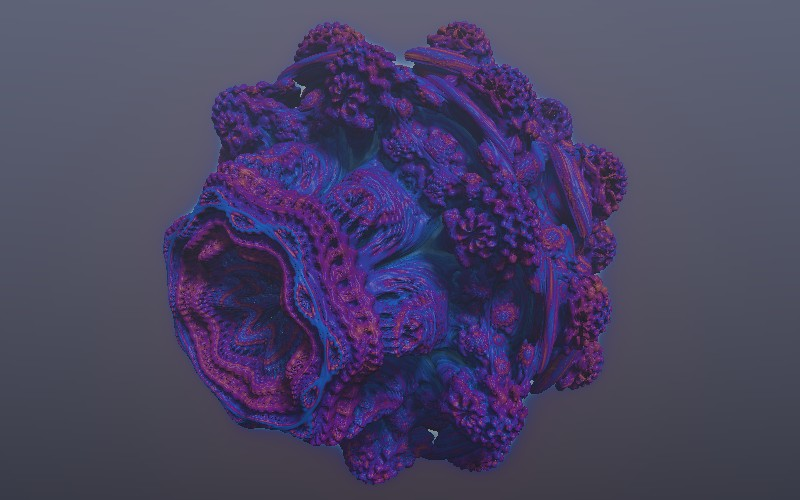
\includegraphics[width=0.88\textwidth]{img/mandelbulb.jpg}
\caption{Mandelbulb, default parameters (8 iterations).}\end{figure}
\paragraph{Parameters (app defaults).} Iterations 8 (range 2--16); step factor 0.9; bounding size 1.2.

{\footnotesize\begin{tabular}{@{}llrr@{}}\toprule Parameter & Key & Default & Range\\\midrule
Power & \texttt{power} & 8 & 2\,\dots\,16\\
Theta phase & \texttt{theta} & 0$^\circ$ & $-$180\,\dots\,180\\
Phi phase & \texttt{phi} & 0$^\circ$ & $-$180\,\dots\,180\\
Julia mix & \texttt{julia} & 0 & 0\,\dots\,1\\
Julia c x & \texttt{cx} & 0.35 & $-$1.5\,\dots\,1.5\\
Julia c y & \texttt{cy} & 0.3 & $-$1.5\,\dots\,1.5\\
Julia c z & \texttt{cz} & $-$0.4 & $-$1.5\,\dots\,1.5\\
\bottomrule\end{tabular}}


\subsection{Quaternion Julia}
A 3D slice of the 4D Julia set of $q\mapsto q^2+\vv c$ for quaternions. Write $\vv z=(z_w; \vv v)$ with real part $z_w$ and vector part $\vv v\in\R^3$.
Start at $\vv z_0=(p_x,p_y,p_z,w_0)$ where $w_0$ is the \emph{4D slice} parameter:
\begin{align}
\vv z_{k+1}&=\big(z_x^2-\norm{(z_y,z_z,z_w)}^2,\ 2z_x\,(z_y,z_z,z_w)\big)+\vv c,\quad \vv c=(c_x,c_y,c_z,c_w),\\
\mathrm{md2}_{k+1}&=4\norm{\vv z_k}^2\,\mathrm{md2}_k,\qquad\mathrm{md2}_0=1\quad(\text{squared derivative norm}),\\
\DE&=\tfrac14\sqrt{\frac{\norm{\vv z}^2}{\mathrm{md2}}}\;\ln\norm{\vv z}^2.
\end{align}
Escape when $\norm{\vv z}^2>16$.
\begin{figure}[H]\centering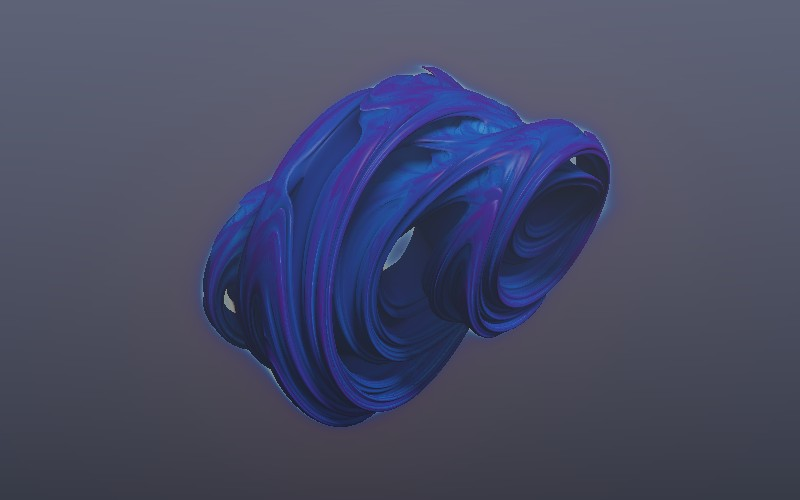
\includegraphics[width=0.88\textwidth]{img/julia.jpg}
\caption{Quaternion Julia, default parameters (11 iterations).}\end{figure}
\paragraph{Parameters (app defaults).} Iterations 11 (range 2--20); step factor 0.9; bounding size 1.3.

{\footnotesize\begin{tabular}{@{}llrr@{}}\toprule Parameter & Key & Default & Range\\\midrule
c x & \texttt{cx} & $-$0.291 & $-$1.5\,\dots\,1.5\\
c y & \texttt{cy} & $-$0.399 & $-$1.5\,\dots\,1.5\\
c z & \texttt{cz} & 0.339 & $-$1.5\,\dots\,1.5\\
c w & \texttt{cw} & 0.437 & $-$1.5\,\dots\,1.5\\
4D slice & \texttt{slice} & 0 & $-$1\,\dots\,1\\
\bottomrule\end{tabular}}


\subsection{Folded bulb hybrid}
A Mandelbulb whose orbit is mirror-folded and rotated before every $e$-th iteration (\emph{Fold every}). With fold amount $\mu\in[0,1]$:
\begin{align}
\text{if } k\bmod e=0:&\quad \vv z\leftarrow\Rot_A\big((1-\mu)\vv z+\mu\abs{\vv z}\big),\\
&\quad \mathrm{dr}\leftarrow n\,r^{n-1}\mathrm{dr}+1,\qquad \vv z\leftarrow\mathcal B_n(\vv z)+\vv p,
\end{align}
with $r=\norm{\vv z}$ evaluated after the fold. Escape at $r>2$, and $\DE=\tfrac12\,r\ln r/\abs{\mathrm{dr}}$.
$\mu=0$ is the plain bulb; $\mu=1$ is a full mirror fold.
\begin{figure}[H]\centering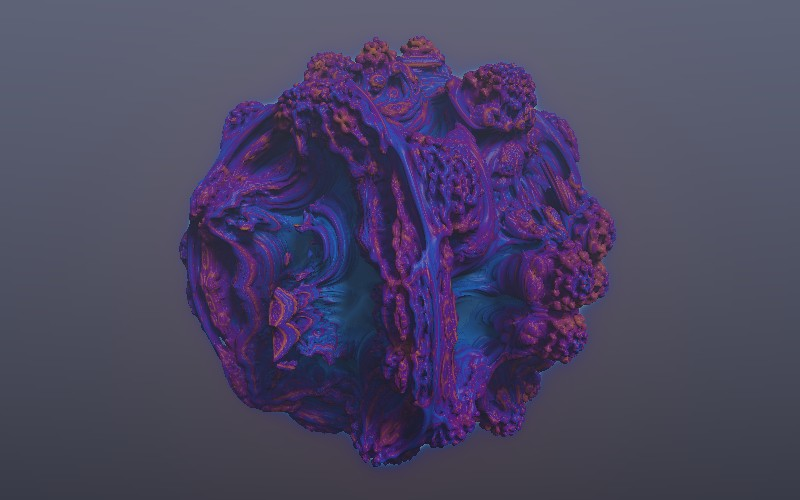
\includegraphics[width=0.88\textwidth]{img/hybrid.jpg}
\caption{Folded bulb hybrid, default parameters (9 iterations).}\end{figure}
\paragraph{Parameters (app defaults).} Iterations 9 (range 2--20); step factor 0.85; bounding size 1.3.

{\footnotesize\begin{tabular}{@{}llrr@{}}\toprule Parameter & Key & Default & Range\\\midrule
Bulb power & \texttt{power} & 8 & 2\,\dots\,12\\
Fold amount & \texttt{fold} & 1 & 0\,\dots\,1\\
Fold every & \texttt{every} & 1 & 1\,\dots\,4\\
Rotation X & \texttt{rotX} & 0$^\circ$ & $-$180\,\dots\,180\\
Rotation Y & \texttt{rotY} & 30$^\circ$ & $-$180\,\dots\,180\\
Rotation Z & \texttt{rotZ} & 15$^\circ$ & $-$180\,\dots\,180\\
\bottomrule\end{tabular}}


% =====================================================================
\section{Mandelbox family (box fold + sphere fold)}
All of these iterate $\vv z\leftarrow s\,\vv z+\vv p$ after folding, with $\mathrm{dr}\leftarrow\abs s\,\mathrm{dr}+1$, and
return $\DE=\norm{\vv z}/\abs{\mathrm{dr}}$ (escape when $\norm{\vv z}^2>10^4$). Negative $s$ gives compact boxes, positive $s$ open lattices.

\subsection{Mandelbox}
\begin{align}
\vv z&\leftarrow\bfold_f(\vv z),\qquad (\vv z,\mathrm{dr})\leftarrow\sfold_{m,R}(\vv z,\mathrm{dr}),\\
\vv z&\leftarrow s\vv z+\vv p,\qquad\mathrm{dr}\leftarrow\abs s\,\mathrm{dr}+1,
\end{align}
with $m$ = \emph{Min radius}, $R=\max(\text{Fixed radius},m+0.01)$, $f$ = \emph{Fold limit}.
\begin{figure}[H]\centering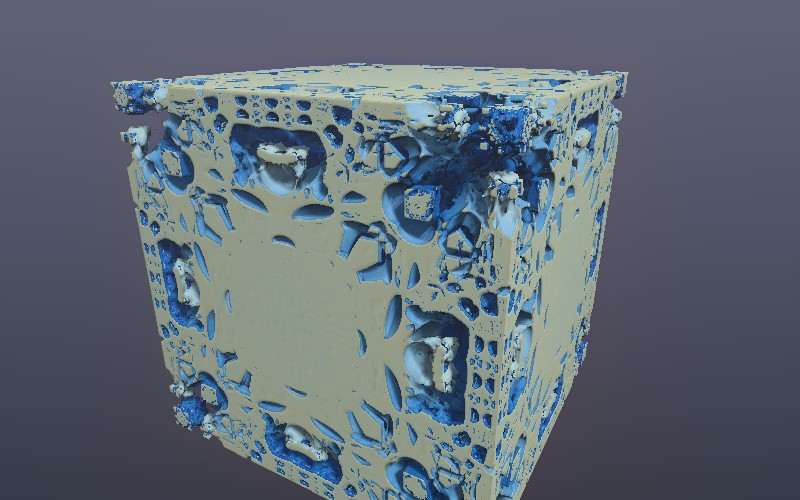
\includegraphics[width=0.88\textwidth]{img/mandelbox.jpg}
\caption{Mandelbox, default parameters (12 iterations).}\end{figure}
\paragraph{Parameters (app defaults).} Iterations 12 (range 2--24); step factor 1; bounding size 3.

{\footnotesize\begin{tabular}{@{}llrr@{}}\toprule Parameter & Key & Default & Range\\\midrule
Scale & \texttt{scale} & $-$1.8 & $-$3\,\dots\,3\\
Min radius & \texttt{minR} & 0.5 & 0.05\,\dots\,1\\
Fixed radius & \texttt{fixedR} & 1 & 0.3\,\dots\,2\\
Fold limit & \texttt{fold} & 1 & 0.3\,\dots\,2\\
\bottomrule\end{tabular}}


\subsection{Amazing Box}
The Mandelbox with fixed $R=1$ and a rotation inserted each iteration (organic, surface-like folds):
\begin{equation}
\vv z\leftarrow\Rot_A\,\sfold_{m,1}\big(\bfold_f(\vv z)\big),\qquad\vv z\leftarrow s\vv z+\vv p.
\end{equation}
\begin{figure}[H]\centering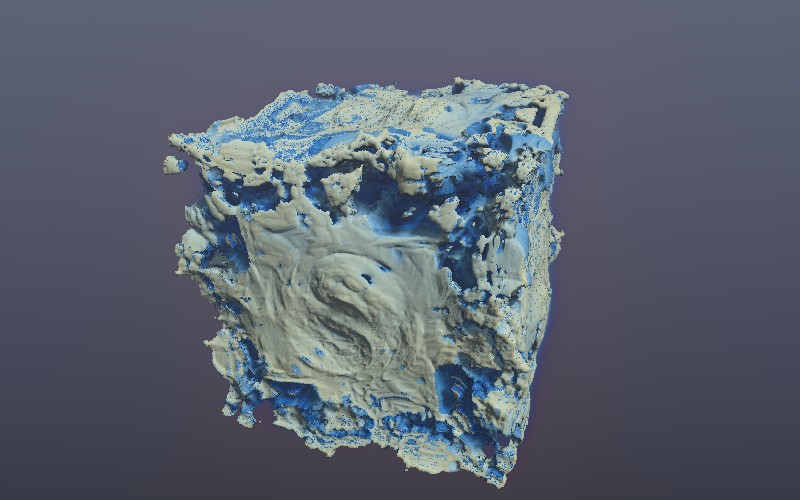
\includegraphics[width=0.88\textwidth]{img/amazingBox.jpg}
\caption{Amazing Box, default parameters (12 iterations).}\end{figure}
\paragraph{Parameters (app defaults).} Iterations 12 (range 2--24); step factor 0.8; bounding size 2.4.

{\footnotesize\begin{tabular}{@{}llrr@{}}\toprule Parameter & Key & Default & Range\\\midrule
Scale & \texttt{scale} & $-$1.7 & $-$3\,\dots\,3\\
Min radius & \texttt{minR} & 0.35 & 0.05\,\dots\,1\\
Fold limit & \texttt{fold} & 1 & 0.3\,\dots\,2\\
Rotation X & \texttt{rotX} & 12$^\circ$ & $-$180\,\dots\,180\\
Rotation Y & \texttt{rotY} & 0$^\circ$ & $-$180\,\dots\,180\\
Rotation Z & \texttt{rotZ} & 20$^\circ$ & $-$180\,\dots\,180\\
\bottomrule\end{tabular}}


\subsection{Vaulted box}
Mandelbox with independent fold limits on the horizontal ($f$) and vertical ($f_y$) axes, and a sphere fold whose radius is blended towards a \emph{cylinder} along $z$ by the vault amount $v\in[0,1]$:
\begin{align}
\vv z_{xz}&\leftarrow\bfold_f(\vv z_{xz}),\quad z_y\leftarrow\bfold_{f_y}(z_y),\\
r^2&=(1-v)\,\norm{\vv z}^2+v\,\norm{\vv z_{xy}}^2,\qquad
k=\begin{cases}1/m^2&r<m\\1/r^2&m\le r<1\\1&\text{else}\end{cases},\\
\vv z&\leftarrow\Rot_A(k\vv z),\ \ \mathrm{dr}\leftarrow k\,\mathrm{dr},\qquad \vv z\leftarrow s\vv z+\vv p.
\end{align}
$v=0$ is the Mandelbox; $v=1$ gives barrel vaults running along $z$.
\begin{figure}[H]\centering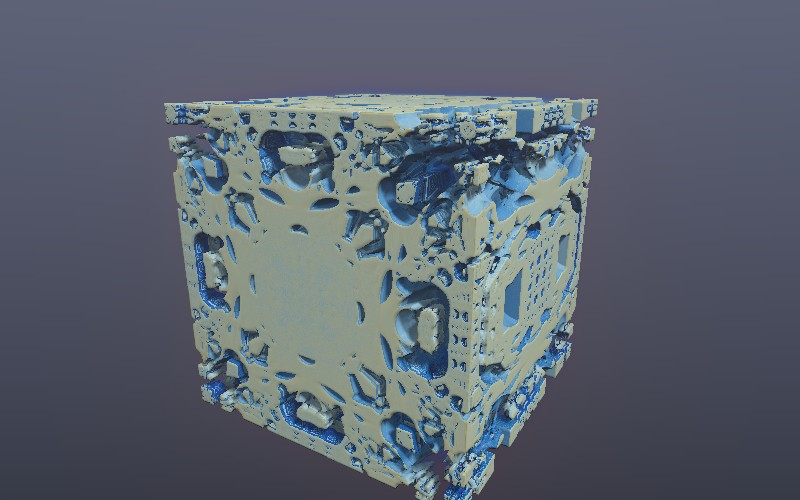
\includegraphics[width=0.88\textwidth]{img/vaulted.jpg}
\caption{Vaulted box, default parameters (12 iterations).}\end{figure}
\paragraph{Parameters (app defaults).} Iterations 12 (range 2--24); step factor 0.8; bounding size 3.

{\footnotesize\begin{tabular}{@{}llrr@{}}\toprule Parameter & Key & Default & Range\\\midrule
Scale & \texttt{scale} & $-$1.8 & $-$3\,\dots\,3\\
Min radius & \texttt{minR} & 0.45 & 0.05\,\dots\,1\\
Fold limit & \texttt{fold} & 1 & 0.3\,\dots\,2\\
Height fold & \texttt{foldY} & 1 & 0.3\,\dots\,2\\
Vault & \texttt{vault} & 0.8 & 0\,\dots\,1\\
Rotation X & \texttt{rotX} & 0$^\circ$ & $-$180\,\dots\,180\\
Rotation Y & \texttt{rotY} & 0$^\circ$ & $-$180\,\dots\,180\\
Rotation Z & \texttt{rotZ} & 0$^\circ$ & $-$180\,\dots\,180\\
\bottomrule\end{tabular}}


\subsection{Amazing Surf}
Like Amazing Box but the box fold acts on $x,z$ only, leaving $y$ unfolded, and an additive lift $\ell$ on $y$ bends the sheets:
\begin{align}
\vv z_{xz}&\leftarrow\bfold_f(\vv z_{xz}),\qquad(\vv z,\mathrm{dr})\leftarrow\sfold_{m,1}(\vv z,\mathrm{dr}),\\
\vv z&\leftarrow s\,\Rot_A\vv z+\vv p+(0,\ell,0)^{\!\top}.
\end{align}
\begin{figure}[H]\centering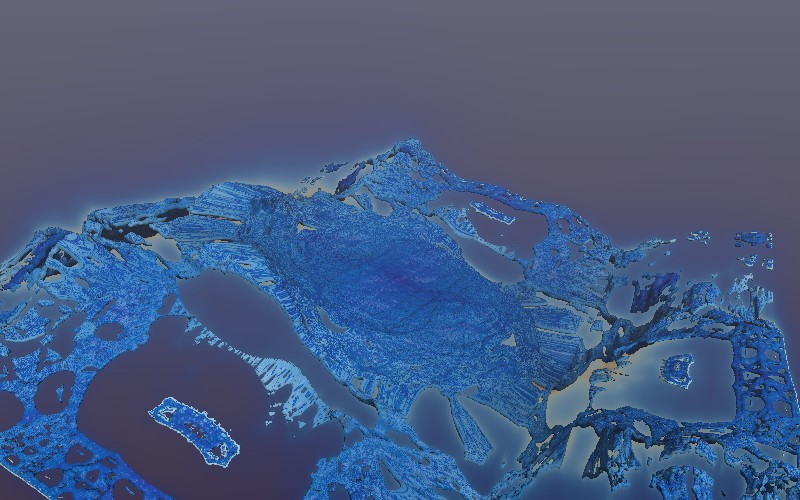
\includegraphics[width=0.88\textwidth]{img/amazingSurf.jpg}
\caption{Amazing Surf, default parameters (10 iterations).}\end{figure}
\paragraph{Parameters (app defaults).} Iterations 10 (range 2--20); step factor 0.6; bounding size 1.6; \emph{unbounded} (no bounding sphere assumed).

{\footnotesize\begin{tabular}{@{}llrr@{}}\toprule Parameter & Key & Default & Range\\\midrule
Scale & \texttt{scale} & $-$1.75 & $-$3\,\dots\,3\\
Min radius & \texttt{minR} & 0.45 & 0.05\,\dots\,1\\
Fold limit & \texttt{fold} & 1 & 0.3\,\dots\,2\\
Sheet lift & \texttt{lift} & 0 & $-$1\,\dots\,1\\
Rotation X & \texttt{rotX} & 6$^\circ$ & $-$180\,\dots\,180\\
Rotation Y & \texttt{rotY} & 0$^\circ$ & $-$180\,\dots\,180\\
Rotation Z & \texttt{rotZ} & 9$^\circ$ & $-$180\,\dots\,180\\
\bottomrule\end{tabular}}


\subsection{KaliBox}
Kali's abs-fold set, carried as a 4-vector $\vv Z=(\vv z,w)$ with $w_0=1$ tracking the scale. With $m$ = \emph{Min radius}$^2$, shift $\vv t$, Julia offset $\vv c=(c_x,c_y,c_z,0)$:
\begin{align}
\vv z&\leftarrow\abs{\vv z}+\vv t,\qquad r^2=\norm{\vv z}^2,\\
\vv Z&\leftarrow\vv Z\cdot\min\!\big(1,\max(m/r^2,\,m)\big)\quad\Big(=1\text{ if }r^2\le m;\ m/r^2\text{ if }m<r^2<1;\ m\text{ if }r^2\ge 1\Big),\\
\vv Z&\leftarrow\frac{s}{m}\vv Z+\vv c,\qquad\vv z\leftarrow\Rot_A\vv z.
\end{align}
After $N$ iterations:
\begin{equation}\DE=\frac{\norm{\vv z}-\abs{s-1}}{\abs w}-\abs s^{\,1-N}.\end{equation}
\begin{figure}[H]\centering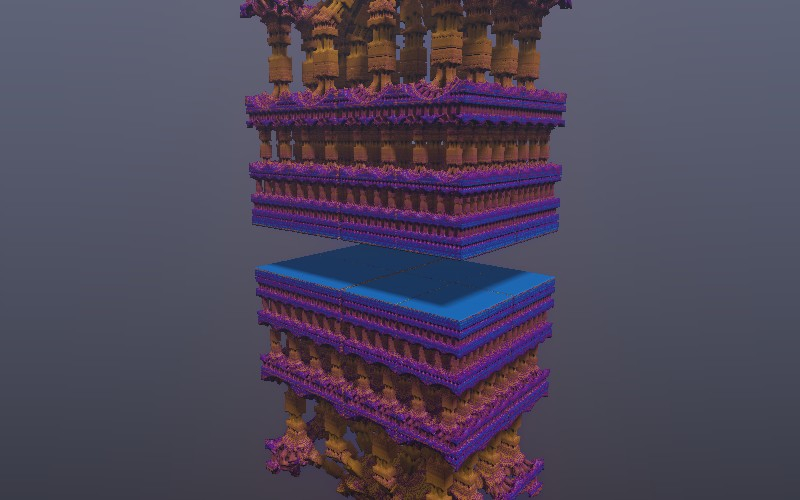
\includegraphics[width=0.88\textwidth]{img/kaliBox.jpg}
\caption{KaliBox, default parameters (13 iterations).}\end{figure}
\paragraph{Parameters (app defaults).} Iterations 13 (range 2--24); step factor 0.7; bounding size 2.2.

{\footnotesize\begin{tabular}{@{}llrr@{}}\toprule Parameter & Key & Default & Range\\\midrule
Scale & \texttt{scale} & 2.043 & 1.2\,\dots\,3\\
Min radius$^2$ & \texttt{minR2} & 0.349 & 0.05\,\dots\,1\\
Shift X & \texttt{tx} & 0.036 & $-$2\,\dots\,2\\
Shift Y & \texttt{ty} & $-$1.861 & $-$2.5\,\dots\,1\\
Shift Z & \texttt{tz} & 0.036 & $-$2\,\dots\,2\\
Julia X & \texttt{jx} & $-$0.669 & $-$1.5\,\dots\,1.5\\
Julia Y & \texttt{jy} & $-$1.303 & $-$1.5\,\dots\,1.5\\
Julia Z & \texttt{jz} & $-$0.458 & $-$1.5\,\dots\,1.5\\
Rotation X & \texttt{rotX} & 0$^\circ$ & $-$180\,\dots\,180\\
Rotation Y & \texttt{rotY} & 0$^\circ$ & $-$180\,\dots\,180\\
Rotation Z & \texttt{rotZ} & 0$^\circ$ & $-$180\,\dots\,180\\
\bottomrule\end{tabular}}


\subsection{Pseudo-Kleinian}
Knighty's limit set of a Kleinian-like group: a box fold with half-extents $\vv c_s=(a,a,b)$ followed by a one-sided sphere inversion of size $S$ and a translation $\vv c$:
\begin{align}
\vv z&\leftarrow 2\clamp(\vv z,-\vv c_s,\vv c_s)-\vv z,\qquad r^2=\norm{\vv z}^2,\\
k&=\max\!\big(S/r^2,\,1\big),\quad\vv z\leftarrow k\vv z+\vv c,\quad\mathrm{dr}\leftarrow k\,\mathrm{dr}.
\end{align}
With $\rho=\norm{\vv z_{xy}}$ and strut radius $t$:
\begin{equation}\DE=\frac{\max\!\Big(\rho-t,\ \dfrac{\abs{\rho\,z_z}}{\norm{\vv z}}\Big)}{\mathrm{dr}}.\end{equation}
\begin{figure}[H]\centering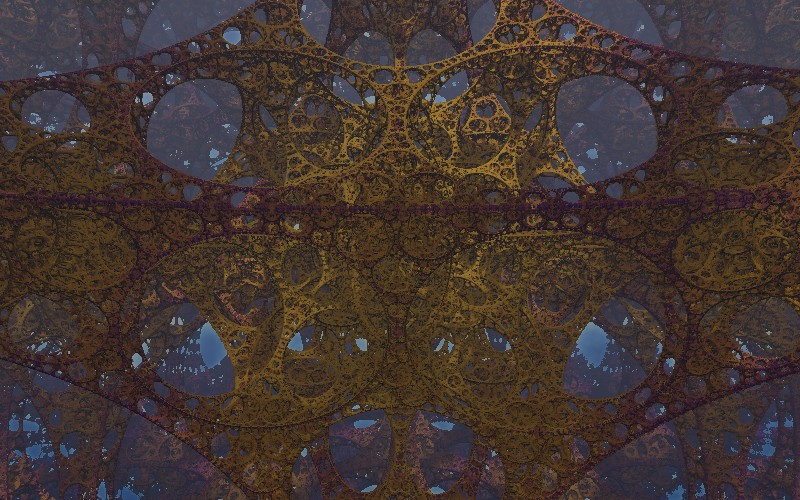
\includegraphics[width=0.88\textwidth]{img/pseudoKleinian.jpg}
\caption{Pseudo-Kleinian, default parameters (9 iterations).}\end{figure}
\paragraph{Parameters (app defaults).} Iterations 9 (range 2--20); step factor 0.8; bounding size 1; \emph{unbounded} (no bounding sphere assumed).

{\footnotesize\begin{tabular}{@{}llrr@{}}\toprule Parameter & Key & Default & Range\\\midrule
Box width & \texttt{boxXY} & 0.908 & 0.4\,\dots\,1.4\\
Box height & \texttt{boxZ} & 0.924 & 0.4\,\dots\,1.6\\
Inversion size & \texttt{size} & 1 & 0.6\,\dots\,1.6\\
Offset X & \texttt{cx} & 0 & $-$0.5\,\dots\,0.5\\
Offset Y & \texttt{cy} & 0 & $-$0.5\,\dots\,0.5\\
Offset Z & \texttt{cz} & 0 & $-$0.5\,\dots\,0.5\\
Thickness & \texttt{thick} & 0.928 & 0.5\,\dots\,1.2\\
\bottomrule\end{tabular}}


\subsection{Apollonian}
Infinite sphere-inversion lattice. Per iteration, fold space into the cell $[-1,1]^3$ and invert:
\begin{align}
\vv z&\leftarrow-1+2\,\fract\!\big(\tfrac12\vv z+\tfrac12\big),\qquad r^2=\norm{\vv z}^2,\\
f&=\frac{k}{\max(r^2,10^{-6})},\quad\vv z\leftarrow f\vv z,\quad \mathrm{sc}\leftarrow f\,\mathrm{sc},\qquad\DE=\frac{\abs{z_y}}{4\,\mathrm{sc}}.
\end{align}
$k$ = \emph{Inversion size}; the lattice is unbounded (use the bound radius to cut it out).
\begin{figure}[H]\centering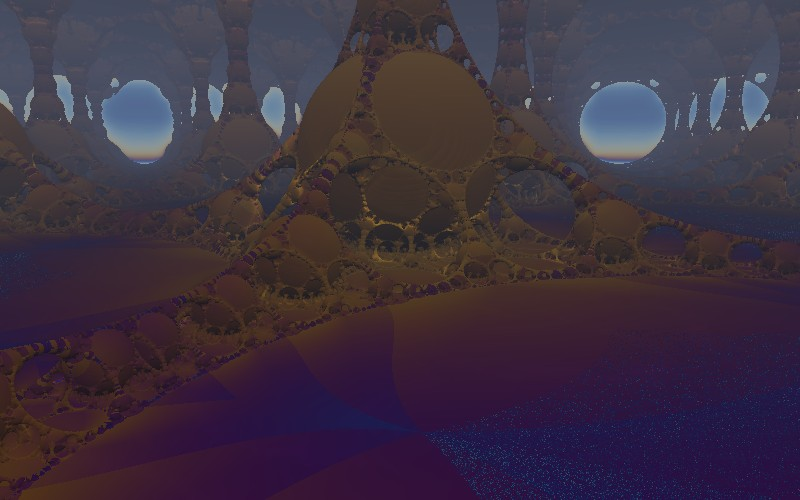
\includegraphics[width=0.88\textwidth]{img/apollonian.jpg}
\caption{Apollonian, default parameters (8 iterations).}\end{figure}
\paragraph{Parameters (app defaults).} Iterations 8 (range 2--14); step factor 1; bounding size 1; \emph{unbounded} (no bounding sphere assumed).

{\footnotesize\begin{tabular}{@{}llrr@{}}\toprule Parameter & Key & Default & Range\\\midrule
Inversion size & \texttt{k} & 1.15 & 0.8\,\dots\,1.6\\
\bottomrule\end{tabular}}


% =====================================================================
\section{Kaleidoscopic IFS (fold, rotate, scale)}
These are \emph{iterated function systems}: instead of an escape test, each iteration applies a fold, a rotation and a scaling about an offset. They share
$\mathrm{dr}_{k+1}=s\,\mathrm{dr}_k$, and the distance is that of a simple shape in the final folded frame, divided by $\mathrm{dr}$.

\subsection{Menger KIFS}
\begin{align}
\vv z&\leftarrow\sortd(\abs{\vv z}),\qquad\vv z\leftarrow S_{s,\vv o}(\Rot_A\vv z),\\
&\text{if }z_z<-\tfrac12 o_z(s-1):\quad z_z\leftarrow z_z+o_z(s-1),\\
\DE&=\sdbox(\vv z,\,(1,1,1))\,/\,s^{N}.
\end{align}
With $s=3$, $\vv o=(1,1,1)$, no rotation, this is the exact Menger sponge.
\begin{figure}[H]\centering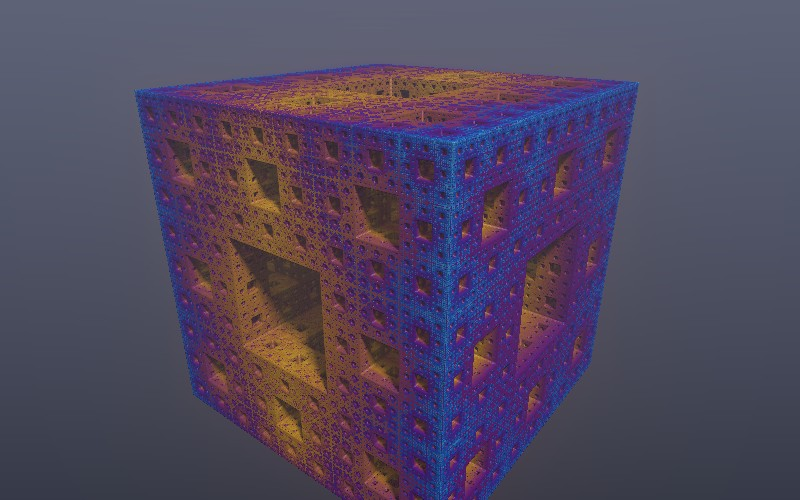
\includegraphics[width=0.88\textwidth]{img/kifsMenger.jpg}
\caption{Menger KIFS, default parameters (6 iterations).}\end{figure}
\paragraph{Parameters (app defaults).} Iterations 6 (range 2--12); step factor 1; bounding size 1.4.

{\footnotesize\begin{tabular}{@{}llrr@{}}\toprule Parameter & Key & Default & Range\\\midrule
Scale & \texttt{scale} & 3 & 2\,\dots\,4\\
Offset X & \texttt{offX} & 1 & 0\,\dots\,2\\
Offset Y & \texttt{offY} & 1 & 0\,\dots\,2\\
Offset Z & \texttt{offZ} & 1 & 0\,\dots\,2\\
Rotation X & \texttt{rotX} & 0$^\circ$ & $-$180\,\dots\,180\\
Rotation Y & \texttt{rotY} & 0$^\circ$ & $-$180\,\dots\,180\\
Rotation Z & \texttt{rotZ} & 0$^\circ$ & $-$180\,\dots\,180\\
\bottomrule\end{tabular}}


\subsection{Sierpinski}
Tetrahedral folds (reflections in the planes $x+y=0$, $x+z=0$, $y+z=0$):
\begin{align}
&x+y<0:\ (x,y)\leftarrow(-y,-x);\quad x+z<0:\ (x,z)\leftarrow(-z,-x);\quad y+z<0:\ (y,z)\leftarrow(-z,-y),\\
&\vv z\leftarrow S_{s,\vv o}(\Rot_A\vv z),\quad\vv o=(o,o,o),\qquad\DE=\big(\norm{\vv z}-1\big)/s^{N}.
\end{align}
\begin{figure}[H]\centering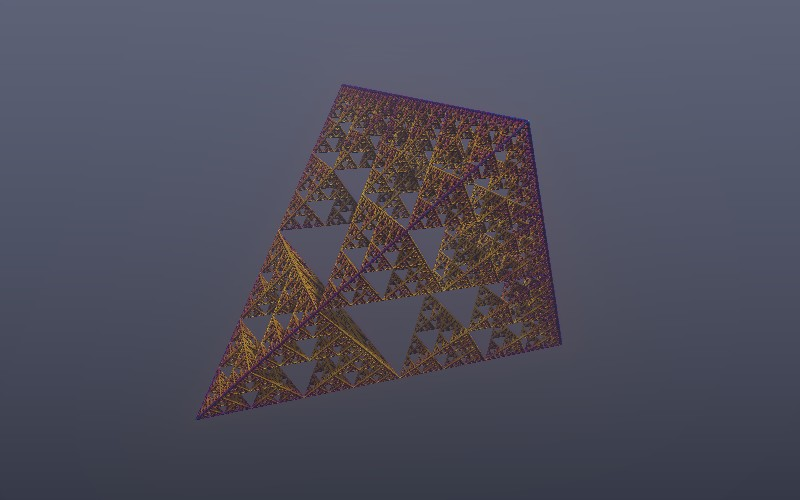
\includegraphics[width=0.88\textwidth]{img/sierpinski.jpg}
\caption{Sierpinski, default parameters (12 iterations).}\end{figure}
\paragraph{Parameters (app defaults).} Iterations 12 (range 2--20); step factor 1; bounding size 1.6.

{\footnotesize\begin{tabular}{@{}llrr@{}}\toprule Parameter & Key & Default & Range\\\midrule
Scale & \texttt{scale} & 2 & 1.5\,\dots\,3\\
Offset & \texttt{offset} & 1 & 0.3\,\dots\,1.6\\
Rotation X & \texttt{rotX} & 0$^\circ$ & $-$180\,\dots\,180\\
Rotation Y & \texttt{rotY} & 0$^\circ$ & $-$180\,\dots\,180\\
Rotation Z & \texttt{rotZ} & 0$^\circ$ & $-$180\,\dots\,180\\
\bottomrule\end{tabular}}


\subsection{Octahedral KIFS}
\begin{equation}
\vv z\leftarrow S_{s,\vv o}\big(\Rot_A\,\sortd(\abs{\vv z})\big),\qquad\DE=\big(\norm{\vv z}-1\big)/s^{N}.
\end{equation}
\begin{figure}[H]\centering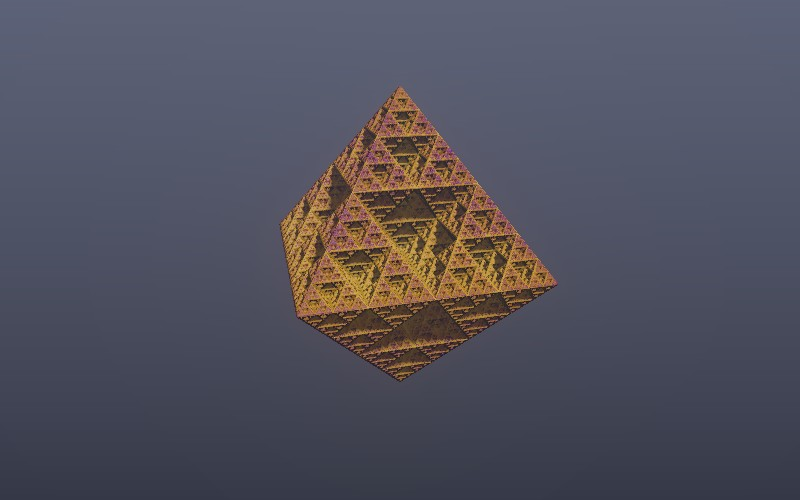
\includegraphics[width=0.88\textwidth]{img/octahedra.jpg}
\caption{Octahedral KIFS, default parameters (12 iterations).}\end{figure}
\paragraph{Parameters (app defaults).} Iterations 12 (range 2--20); step factor 1; bounding size 1.8.

{\footnotesize\begin{tabular}{@{}llrr@{}}\toprule Parameter & Key & Default & Range\\\midrule
Scale & \texttt{scale} & 2 & 1.5\,\dots\,3.5\\
Offset X & \texttt{offX} & 1 & 0\,\dots\,2\\
Offset Y & \texttt{offY} & 0 & 0\,\dots\,2\\
Offset Z & \texttt{offZ} & 0 & 0\,\dots\,2\\
Rotation X & \texttt{rotX} & 0$^\circ$ & $-$180\,\dots\,180\\
Rotation Y & \texttt{rotY} & 0$^\circ$ & $-$180\,\dots\,180\\
Rotation Z & \texttt{rotZ} & 0$^\circ$ & $-$180\,\dots\,180\\
\bottomrule\end{tabular}}


\subsection{Kaleidoscopic IFS}
Two rotations around the same fold:
\begin{equation}
\vv z\leftarrow S_{s,\vv o}\Big(\Rot_B\,\sortd\big(\abs{\Rot_A\vv z}\big)\Big),\qquad\DE=\big(\norm{\vv z}-1\big)/s^{N}.
\end{equation}
$\Rot_A$ = pre-rotation, $\Rot_B$ = post-rotation.
\begin{figure}[H]\centering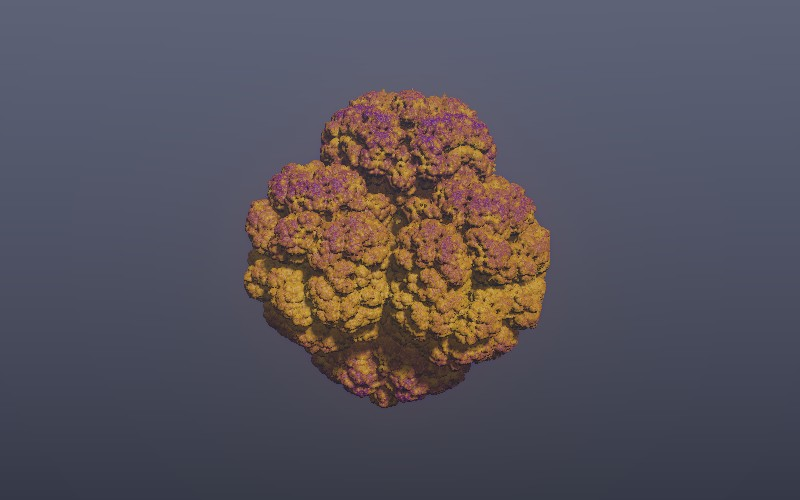
\includegraphics[width=0.88\textwidth]{img/kaleidoscopic.jpg}
\caption{Kaleidoscopic IFS, default parameters (12 iterations).}\end{figure}
\paragraph{Parameters (app defaults).} Iterations 12 (range 2--20); step factor 0.9; bounding size 1.8.

{\footnotesize\begin{tabular}{@{}llrr@{}}\toprule Parameter & Key & Default & Range\\\midrule
Scale & \texttt{scale} & 2.4 & 1.4\,\dots\,3.5\\
Offset X & \texttt{offX} & 1 & 0\,\dots\,2\\
Offset Y & \texttt{offY} & 0.5 & 0\,\dots\,2\\
Offset Z & \texttt{offZ} & 0.25 & 0\,\dots\,2\\
Pre-rotation X & \texttt{preX} & 10$^\circ$ & $-$180\,\dots\,180\\
Pre-rotation Y & \texttt{preY} & 20$^\circ$ & $-$180\,\dots\,180\\
Pre-rotation Z & \texttt{preZ} & 0$^\circ$ & $-$180\,\dots\,180\\
Post-rotation X & \texttt{postX} & 0$^\circ$ & $-$180\,\dots\,180\\
Post-rotation Y & \texttt{postY} & 0$^\circ$ & $-$180\,\dots\,180\\
Post-rotation Z & \texttt{postZ} & 15$^\circ$ & $-$180\,\dots\,180\\
\bottomrule\end{tabular}}


\subsection{Icosahedral KIFS}
Uses Knighty's polyhedral fold for icosahedral symmetry. Let $c=\cos(\pi/5)=0.80901699\ldots$ and
$\vv n=(-\tfrac12,\,-c,\,\sqrt{\tfrac34-c^2})$. The fold, applied five times, is
\begin{equation}
\mathcal F(\vv z):\quad\text{repeat 5 times: }\ \vv z_{xy}\leftarrow\abs{\vv z_{xy}},\quad \vv z\leftarrow\vv z-2\min(0,\ \vv z\!\cdot\!\vv n)\,\vv n.
\end{equation}
Iteration:
\begin{equation}\vv z\leftarrow S_{s,\vv o}\Big(\Rot_B\,\mathcal F(\Rot_A\vv z)\Big),\qquad\DE=\big(\norm{\vv z}-1\big)/s^{N}.
\end{equation}
The offset point $\vv o$ lies in the fundamental cell, spanned by a vertex $\vv A=(0,0,1)$, edge midpoint $\vv B\propto(\sigma,0,\tfrac12)$ and face centre $\vv C\propto(0,\sigma,c)$ with $\sigma=\sqrt{\tfrac34-c^2}$:
\begin{equation}\vv o=\mathrm{reach}\cdot\frac{w_A\vv A+w_B\vv B+w_C\vv C}{\norm{w_A\vv A+w_B\vv B+w_C\vv C}}.\end{equation}
\begin{figure}[H]\centering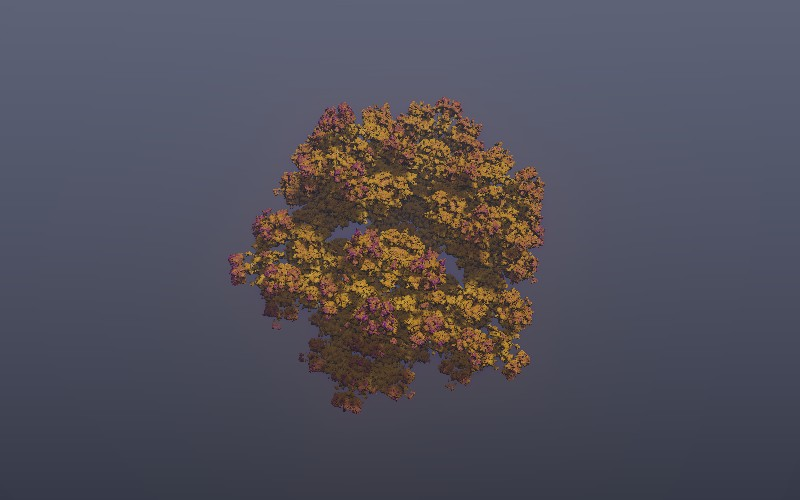
\includegraphics[width=0.88\textwidth]{img/icosahedral.jpg}
\caption{Icosahedral KIFS, default parameters (10 iterations).}\end{figure}
\paragraph{Parameters (app defaults).} Iterations 10 (range 2--20); step factor 0.9; bounding size 1.6.

{\footnotesize\begin{tabular}{@{}llrr@{}}\toprule Parameter & Key & Default & Range\\\midrule
Scale & \texttt{scale} & 2.6 & 1.5\,\dots\,3.5\\
Vertex & \texttt{wA} & 0 & 0\,\dots\,1\\
Edge & \texttt{wB} & 1 & 0\,\dots\,1\\
Face & \texttt{wC} & 0 & 0\,\dots\,1\\
Reach & \texttt{reach} & 1 & 0.2\,\dots\,2\\
Pre-rotation X & \texttt{preX} & 0$^\circ$ & $-$180\,\dots\,180\\
Pre-rotation Y & \texttt{preY} & 8$^\circ$ & $-$180\,\dots\,180\\
Pre-rotation Z & \texttt{preZ} & 0$^\circ$ & $-$180\,\dots\,180\\
Post-rotation X & \texttt{postX} & 0$^\circ$ & $-$180\,\dots\,180\\
Post-rotation Y & \texttt{postY} & 0$^\circ$ & $-$180\,\dots\,180\\
Post-rotation Z & \texttt{postZ} & 12$^\circ$ & $-$180\,\dots\,180\\
\bottomrule\end{tabular}}


\subsection{Hyperbolic honeycomb}
A $\{4,3,n\}$ honeycomb of cubes in the Poincar\'e ball model (here $n$ = \emph{Cubes per edge}, 5 for the compact $\{4,3,5\}$).
Let $R^2=1/\cos(2\pi/n)$ be the squared radius of the cube's face spheres and $D=\sqrt{1+R^2}$ the distance of their centres, which are at $D\,\ex,\ D\,\ey,\ D\,\ez$.

\emph{Travel/drift} is a hyperbolic translation (M\"obius map of the unit ball) that moves the origin to $\vv a=(\text{drift},0,\text{travel})$:
\begin{equation}
T_{\vv a}(\vv x)=\frac{(1+2\vv a\!\cdot\!\vv x+\norm{\vv x}^2)\,\vv a+(1-\norm{\vv a}^2)\,\vv x}{1+2\vv a\!\cdot\!\vv x+\norm{\vv a}^2\norm{\vv x}^2},\qquad
\mathrm{sc}_0=\frac{1-\norm{\vv a}^2}{1+2\vv a\!\cdot\!\vv x+\norm{\vv a}^2\norm{\vv x}^2}.
\end{equation}
Then with $\vv z_0=T_{\vv a}(\vv p)$ and $\vv c_x=D\,\ex$, each iteration folds into the fundamental region and inverts in the face sphere:
\begin{align}
\vv z&\leftarrow\sortd(\abs{\vv z}),\quad\vv v=\vv z-\vv c_x,\quad\text{stop if }\norm{\vv v}^2\ge R^2,\\
k&=R^2/\norm{\vv v}^2,\quad\vv z\leftarrow\vv c_x+k\vv v,\quad\mathrm{sc}\leftarrow k\,\mathrm{sc}.
\end{align}
The edges and vertices are drawn where the inversion spheres meet. With $f_i=\big|\norm{\vv z-D\vv e_i}-R\big|$:
\begin{equation}
d=\min\!\Big(\norm{(f_x,f_y)}-\text{edge},\ \norm{(f_x,f_y,f_z)}-\text{node}\Big),\qquad
\DE=\max\!\Big(\frac{d}{\mathrm{sc}},\ \norm{\vv p}-\text{horizon}\Big).
\end{equation}
\begin{figure}[H]\centering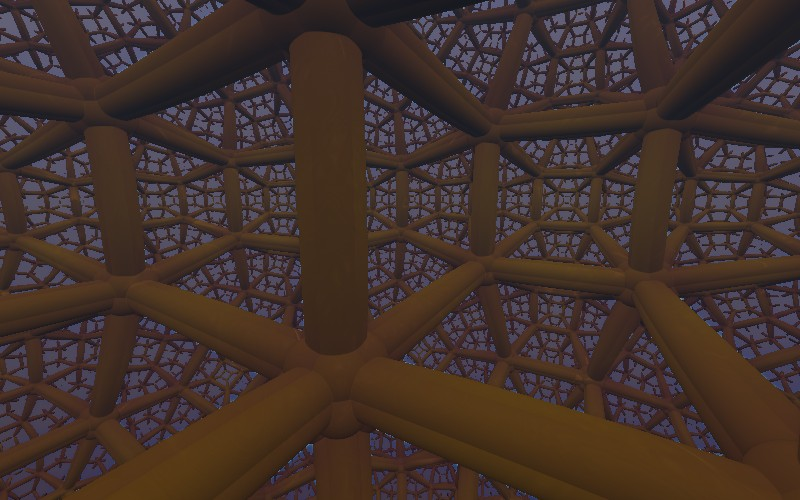
\includegraphics[width=0.88\textwidth]{img/hyperbolic.jpg}
\caption{Hyperbolic honeycomb, default parameters (24 iterations).}\end{figure}
\paragraph{Parameters (app defaults).} Iterations 24 (range 4--32); step factor 0.8; bounding size 1.

{\footnotesize\begin{tabular}{@{}llrr@{}}\toprule Parameter & Key & Default & Range\\\midrule
Cubes per edge & \texttt{order} & 5 & 4.2\,\dots\,8\\
Edge thickness & \texttt{edge} & 0.045 & 0.005\,\dots\,0.2\\
Vertex size & \texttt{node} & 0.08 & 0\,\dots\,0.3\\
Travel & \texttt{travel} & 0 & $-$0.95\,\dots\,0.95\\
Drift & \texttt{drift} & 0 & $-$0.95\,\dots\,0.95\\
Horizon & \texttt{shell} & 0.985 & 0.8\,\dots\,1\\
\bottomrule\end{tabular}}


% =====================================================================
\section{Branching growth (tree, dendrite, nerve cell, root, mycelium, coral)}
\label{sec:branch}
Six formulas share \emph{one} estimator; they differ only in default parameters and in four constants. Each is a \emph{tube that splits, turns and shrinks}.

\paragraph{One generation.} Let $\mathrm{cap}_{h,r}(\vv z)=\norm{\vv z-(0,\clamp(z_y,0,h),0)}-r$ be the distance to a vertical capsule of length $h$ and radius $r$. State: the point $\vv z$ in the current branch's frame, world-up $\vv u$ carried in that frame, accumulated scale $\mathrm{dr}$, current radius $r_k$ (initially $r_0=R$).
\begin{enumerate}
\item \textbf{Measure the branch:} $d\leftarrow\min\!\big(d,\ \mathrm{cap}_{L,r_k}(\vv z)/\mathrm{dr}\big)$.
\item \textbf{Stand at its tip:} $z_y\leftarrow z_y-L$.
\item \textbf{Whorl.} With $N$ branches per node, sector $\varsigma=2\pi/N$ and azimuth $\alpha=\atantwo(z_z,z_x)$, rotate about $y$ into one wedge: $w=\big((\alpha+\varsigma/2)\bmod\varsigma\big)-\varsigma/2$, $\vv z_{xz}\leftarrow\norm{\vv z_{xz}}(\cos w,\sin w)$, and rotate $\vv u$ by the same angle $w-\alpha$. A single capsule now stands for $N$ branches.
\item \textbf{Lean} by the branch angle $\vartheta$ about $z$, then \textbf{twist} by $\psi$ about $y$: $\vv z\leftarrow\Rot_y(\psi)\Rot_z(\vartheta)\vv z$ (same for $\vv u$).
\item \textbf{Droop} $\delta$: with axis $\vv a=\ey\times\vv u/\norm{\ey\times\vv u}$ (skipped if $\vv u\parallel\ey$), $\vv z\leftarrow\Rot_{\vv a}(\delta)\vv z$, $\vv u\leftarrow\Rot_{\vv a}(\delta)\vv u$ (Rodrigues rotation). This bends every branch towards world-down.
\item \textbf{Child frame:} $\vv z\leftarrow\vv z/\varsigma_h$, $\ \mathrm{dr}\leftarrow\mathrm{dr}/\varsigma_h$, $\ r_{k+1}=\kappa\,r_k$, with $\varsigma_h$ = \emph{Shrink} (clamped $\ge0.2$) and $\kappa$ = \emph{Taper}.
\end{enumerate}
Because every step is a rotation or uniform scale (conformal), dividing by $\mathrm{dr}$ gives a true distance \emph{as long as each subtree stays inside its wedge}; for wide angles it can overestimate, which is why the default step factor is $0.35$ and the iteration limit is held at 10. An $N$-way, 11-generation tree has $N^{11}$ twigs but costs only 11 capsule evaluations.

\paragraph{Variants.}
\begin{itemize}
\item \textbf{Root system:} the same with $y\to-y$ at the start (a tree grown downward) and strong droop (``gravity'').
\item \textbf{Nerve cell:} fixed $\kappa=0.95$, no droop, plus a soma sphere $\norm{\vv p}-\rho_s$ and one long unbranched \emph{axon} $\mathrm{cap}_{A,\,0.9R}(p_x,-p_y,p_z)$ downward; $d$ is minimised with both.
\item \textbf{Tree, dendrite, mycelium, coral:} taper and droop are the user parameters; they differ in the defaults tabulated below.
\end{itemize}

\begin{table}[H]\centering\footnotesize
\begin{tabular}{@{}lrrrrrrrr@{}}\toprule
 & Shrink & Angle $\vartheta$ & Twist $\psi$ & $N$ & Seg.\ $L$ & Radius $R$ & Taper $\kappa$ & Droop $\delta$\\\midrule
Tree & 0.68 & 32$^\circ$ & 72$^\circ$ & 4 & 1.00 & 0.110 & 0.86 & 8$^\circ$\\
Dendrite & 0.78 & 64$^\circ$ & 0$^\circ$ & 4 & 1.15 & 0.060 & 1.00 & 0$^\circ$\\
Nerve cell & 0.80 & 44$^\circ$ & 96$^\circ$ & 3 & 0.95 & 0.028 & 0.95 (fixed) & 0\\
Root system & 0.72 & 54$^\circ$ & 38$^\circ$ & 5 & 0.90 & 0.075 & 0.92 & 30$^\circ$, $y$ mirrored\\
Mycelium & 0.87 & 36$^\circ$ & 118$^\circ$ & 6 & 1.25 & 0.016 & 1.02 & $-4^\circ$\\
Coral & 0.74 & 52$^\circ$ & 34$^\circ$ & 6 & 0.62 & 0.200 & 0.97 & $-14^\circ$\\
\bottomrule\end{tabular}
\caption{Branching defaults per formula (generated from the source). Nerve cell also has soma $0.26$ and axon $2.6$.}
\end{table}

\subsection{Tree}\begin{figure}[H]\centering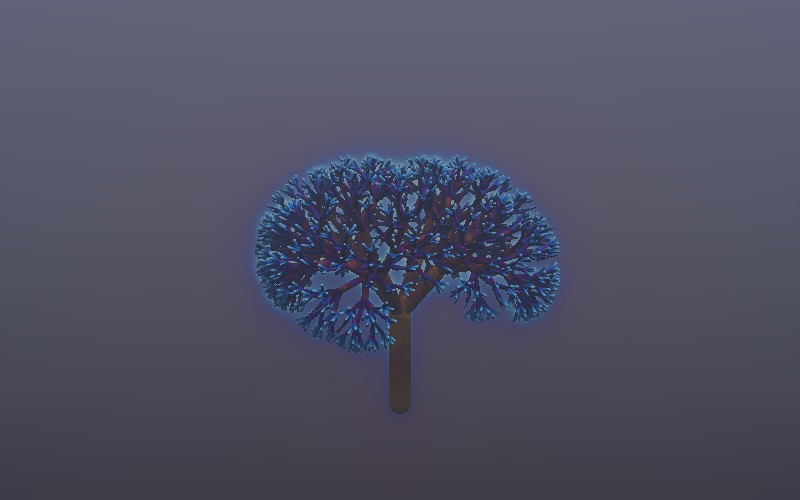
\includegraphics[width=0.88\textwidth]{img/tree.jpg}
\caption{Tree, default parameters (7 iterations).}\end{figure}
\paragraph{Parameters (app defaults).} Iterations 7 (range 3--10); step factor 0.35; bounding size 1.5.

{\footnotesize\begin{tabular}{@{}llrr@{}}\toprule Parameter & Key & Default & Range\\\midrule
Shrink & \texttt{shrink} & 0.68 & 0.45\,\dots\,0.88\\
Branch angle & \texttt{angle} & 32$^\circ$ & 0\,\dots\,85\\
Twist & \texttt{twist} & 72$^\circ$ & $-$180\,\dots\,180\\
Branches & \texttt{folds} & 4 & 2\,\dots\,8\\
Segment & \texttt{len} & 1 & 0.4\,\dots\,2\\
Thickness & \texttt{rad} & 0.11 & 0.02\,\dots\,0.4\\
Taper & \texttt{taper} & 0.86 & 0.5\,\dots\,1.2\\
Droop & \texttt{droop} & 8$^\circ$ & $-$60\,\dots\,60\\
\bottomrule\end{tabular}}

\subsection{Dendrite}\begin{figure}[H]\centering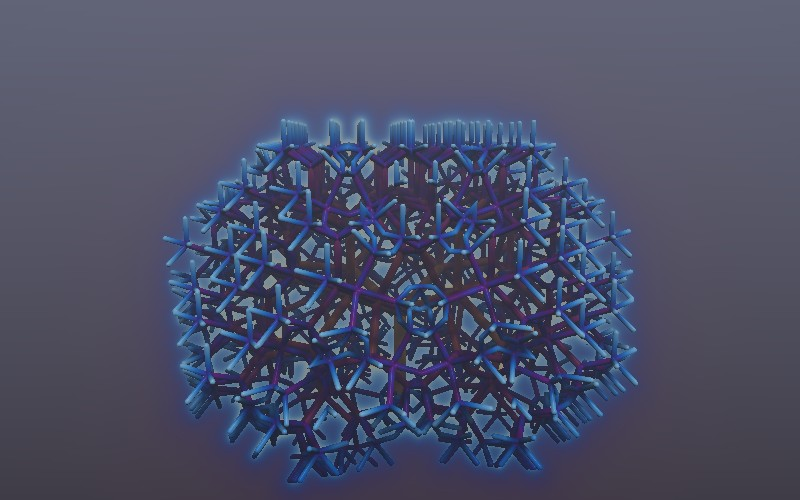
\includegraphics[width=0.88\textwidth]{img/dendrite.jpg}
\caption{Dendrite, default parameters (7 iterations).}\end{figure}
\paragraph{Parameters (app defaults).} Iterations 7 (range 3--10); step factor 0.35; bounding size 1.5.

{\footnotesize\begin{tabular}{@{}llrr@{}}\toprule Parameter & Key & Default & Range\\\midrule
Shrink & \texttt{shrink} & 0.78 & 0.45\,\dots\,0.92\\
Branch angle & \texttt{angle} & 64$^\circ$ & 0\,\dots\,85\\
Twist & \texttt{twist} & 0$^\circ$ & $-$180\,\dots\,180\\
Branches & \texttt{folds} & 4 & 2\,\dots\,8\\
Segment & \texttt{len} & 1.15 & 0.4\,\dots\,2\\
Thickness & \texttt{rad} & 0.06 & 0.02\,\dots\,0.4\\
Taper & \texttt{taper} & 1 & 0.5\,\dots\,1.2\\
Droop & \texttt{droop} & 0$^\circ$ & $-$60\,\dots\,60\\
\bottomrule\end{tabular}}

\subsection{Nerve cell}\begin{figure}[H]\centering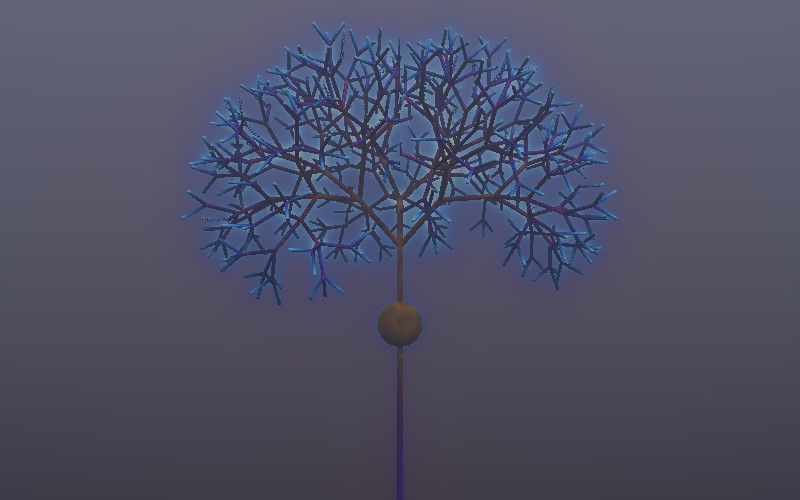
\includegraphics[width=0.88\textwidth]{img/neuron.jpg}
\caption{Nerve cell, default parameters (7 iterations).}\end{figure}
\paragraph{Parameters (app defaults).} Iterations 7 (range 4--10); step factor 0.35; bounding size 1.6.

{\footnotesize\begin{tabular}{@{}llrr@{}}\toprule Parameter & Key & Default & Range\\\midrule
Shrink & \texttt{shrink} & 0.8 & 0.45\,\dots\,0.92\\
Branch angle & \texttt{angle} & 44$^\circ$ & 0\,\dots\,85\\
Twist & \texttt{twist} & 96$^\circ$ & $-$180\,\dots\,180\\
Branches & \texttt{folds} & 3 & 2\,\dots\,8\\
Segment & \texttt{len} & 0.95 & 0.4\,\dots\,2\\
Thickness & \texttt{rad} & 0.028 & 0.01\,\dots\,0.2\\
Cell body & \texttt{soma} & 0.26 & 0\,\dots\,0.6\\
Axon & \texttt{axon} & 2.6 & 0\,\dots\,6\\
\bottomrule\end{tabular}}

\subsection{Root system}\begin{figure}[H]\centering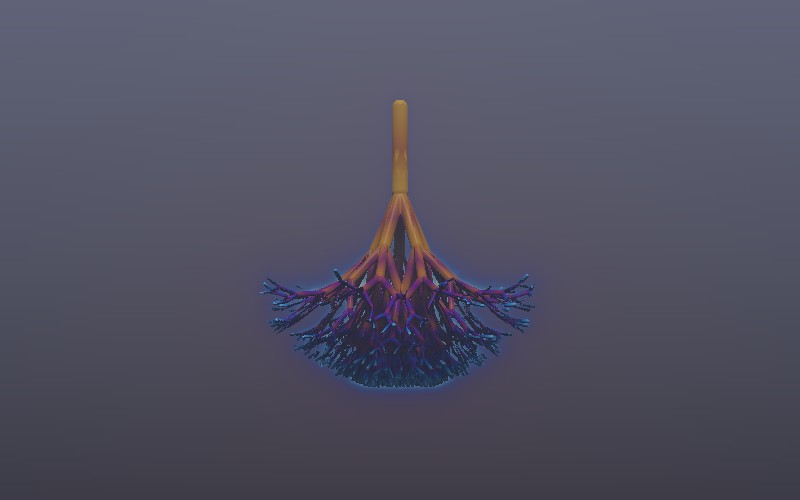
\includegraphics[width=0.88\textwidth]{img/root.jpg}
\caption{Root system, default parameters (7 iterations).}\end{figure}
\paragraph{Parameters (app defaults).} Iterations 7 (range 3--10); step factor 0.35; bounding size 1.5.

{\footnotesize\begin{tabular}{@{}llrr@{}}\toprule Parameter & Key & Default & Range\\\midrule
Shrink & \texttt{shrink} & 0.72 & 0.45\,\dots\,0.9\\
Branch angle & \texttt{angle} & 54$^\circ$ & 0\,\dots\,85\\
Twist & \texttt{twist} & 38$^\circ$ & $-$180\,\dots\,180\\
Branches & \texttt{folds} & 5 & 2\,\dots\,8\\
Segment & \texttt{len} & 0.9 & 0.4\,\dots\,2\\
Thickness & \texttt{rad} & 0.075 & 0.02\,\dots\,0.4\\
Taper & \texttt{taper} & 0.92 & 0.5\,\dots\,1.2\\
Gravity & \texttt{droop} & 30$^\circ$ & $-$60\,\dots\,60\\
\bottomrule\end{tabular}}

\subsection{Mycelium}\begin{figure}[H]\centering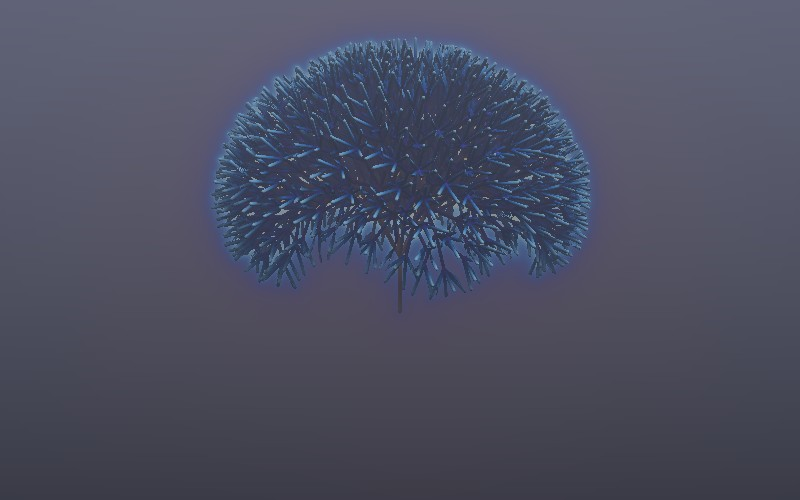
\includegraphics[width=0.88\textwidth]{img/mycelium.jpg}
\caption{Mycelium, default parameters (7 iterations).}\end{figure}
\paragraph{Parameters (app defaults).} Iterations 7 (range 4--10); step factor 0.35; bounding size 1.8; \emph{unbounded} (no bounding sphere assumed).

{\footnotesize\begin{tabular}{@{}llrr@{}}\toprule Parameter & Key & Default & Range\\\midrule
Shrink & \texttt{shrink} & 0.87 & 0.55\,\dots\,0.95\\
Branch angle & \texttt{angle} & 36$^\circ$ & 0\,\dots\,85\\
Twist & \texttt{twist} & 118$^\circ$ & $-$180\,\dots\,180\\
Branches & \texttt{folds} & 6 & 2\,\dots\,8\\
Segment & \texttt{len} & 1.25 & 0.4\,\dots\,2\\
Thickness & \texttt{rad} & 0.016 & 0.005\,\dots\,0.1\\
Taper & \texttt{taper} & 1.02 & 0.6\,\dots\,1.2\\
Drift & \texttt{droop} & $-$4$^\circ$ & $-$60\,\dots\,60\\
\bottomrule\end{tabular}}

\subsection{Coral}\begin{figure}[H]\centering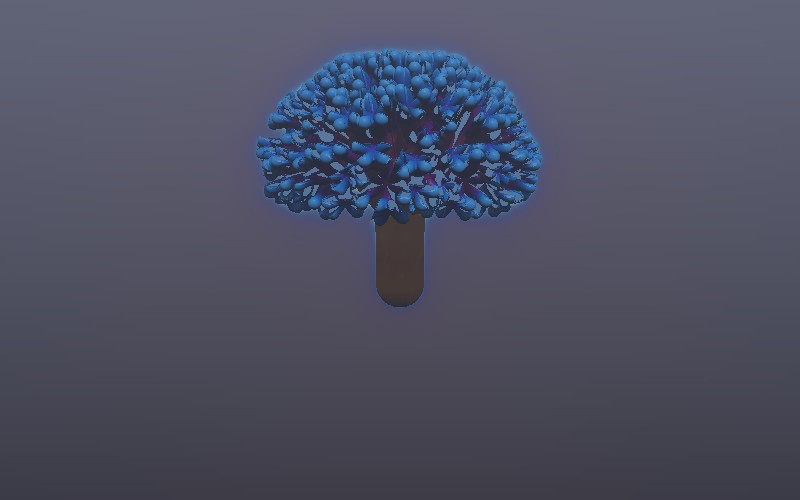
\includegraphics[width=0.88\textwidth]{img/coral.jpg}
\caption{Coral, default parameters (6 iterations).}\end{figure}
\paragraph{Parameters (app defaults).} Iterations 6 (range 3--10); step factor 0.35; bounding size 1.5.

{\footnotesize\begin{tabular}{@{}llrr@{}}\toprule Parameter & Key & Default & Range\\\midrule
Shrink & \texttt{shrink} & 0.74 & 0.45\,\dots\,0.92\\
Branch angle & \texttt{angle} & 52$^\circ$ & 0\,\dots\,85\\
Twist & \texttt{twist} & 34$^\circ$ & $-$180\,\dots\,180\\
Branches & \texttt{folds} & 6 & 2\,\dots\,8\\
Segment & \texttt{len} & 0.62 & 0.4\,\dots\,2\\
Thickness & \texttt{rad} & 0.2 & 0.02\,\dots\,0.4\\
Taper & \texttt{taper} & 0.97 & 0.5\,\dots\,1.2\\
Droop & \texttt{droop} & $-$14$^\circ$ & $-$60\,\dots\,60\\
\bottomrule\end{tabular}}


% =====================================================================
\section{Architecture}

\subsection{Ziggurat}
Four-way folded plan; each generation contributes a stepped pyramid of $T$ tiers. With tier thickness $\vartheta=\text{steepness}/T$ and half-width $w_i=1-0.85\,i/T$:
\begin{align}
\vv z_{xz}&\leftarrow\abs{\vv z_{xz}},\quad\text{if }z_x<z_z:\ \text{swap},\\
p_d&=\min_{i=0}^{T-1}\ \sdbox\!\Big(\vv z-(0,\ \vartheta(i+\tfrac12),\ 0),\ \big(w_i,\ \tfrac12\vartheta,\ w_i\big)\Big),\qquad d\leftarrow\min(d,\ p_d/\mathrm{dr}),\\
\vv z&\leftarrow\Rot_y(\psi)\vv z,\quad \vv z_{xz}\leftarrow s\,\vv z_{xz}-\mathrm{spread}\,(s-1)(1,1),\quad z_y\leftarrow s\,z_y-\mathrm{rise}\,(s-1),\quad\mathrm{dr}\leftarrow s\,\mathrm{dr}.
\end{align}
\begin{figure}[H]\centering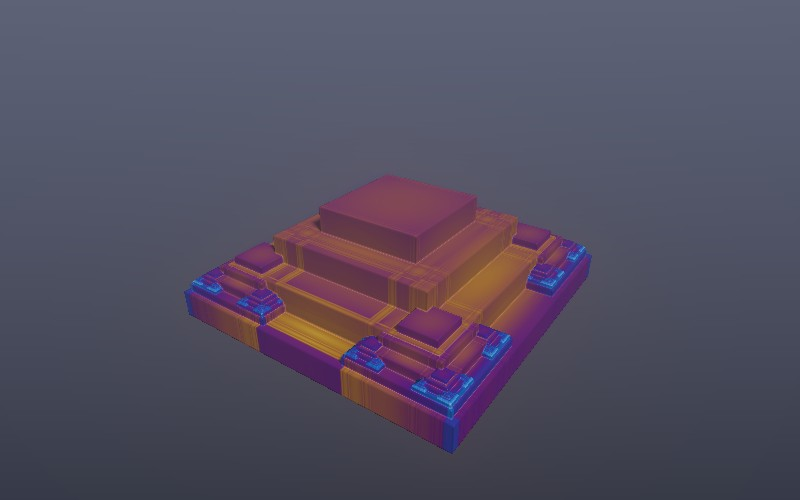
\includegraphics[width=0.88\textwidth]{img/ziggurat.jpg}
\caption{Ziggurat, default parameters (4 iterations).}\end{figure}
\paragraph{Parameters (app defaults).} Iterations 4 (range 1--8); step factor 0.8; bounding size 1.5.

{\footnotesize\begin{tabular}{@{}llrr@{}}\toprule Parameter & Key & Default & Range\\\midrule
Scale & \texttt{scale} & 3 & 2\,\dots\,4\\
Spread & \texttt{spread} & 0.95 & 0\,\dots\,2\\
Rise & \texttt{rise} & 0.25 & $-$1\,\dots\,1\\
Tiers & \texttt{tiers} & 4 & 1\,\dots\,6\\
Steepness & \texttt{steep} & 0.7 & 0.2\,\dots\,2\\
Twist & \texttt{rotY} & 0$^\circ$ & $-$45\,\dots\,45\\
\bottomrule\end{tabular}}


\subsection{Skyline}
\emph{Not a fractal}: a procedural city. Space is cut into blocks of side $c$; block $\vv i=\lfloor p_{xz}/c\rfloor$ may hold a tower, decided by hashes $h_1,h_2,h_3\in[0,1)$ of $\vv i+17\cdot\text{seed}$, where $h(\vv v)=\fract\!\big(P_x P_y\big)$ with $\vv P=\fract(\vv v\odot(123.34,456.21))$ followed by $\vv P\leftarrow\vv P+\vv P\!\cdot(\vv P+45.32)$.
\begin{align}
\text{tower exists}&\iff h_2<\text{density},\qquad H=H_{\max}\big(1-v+v\,1.6\,h_1^2\big),\\
w_x&=\min\!\big(c\,\omega(0.85+0.3h_3),\,0.45c\big),\quad w_z=\min\!\big(w_x'(0.75+0.5h_3),\,0.45c\big),
\end{align}
(with $\omega$ the \emph{tower width}, $w_x'$ before clamping). The tower is a stack of $T$ boxes (tier $k$ of thickness $0.55H\cdot0.6^k$, the last filling up to $H$), each narrowed by $(1-\text{setback})^k$.
The distance considers the block and its eight neighbours (towers never exceed their block): $d=\min\big(p_y,\ \min_{3\times3}\mathrm{tower}\big)$, then clipped to the 3$\times$3 patch edge by $\min(d,\ \min(1.5c-\abs{q_x},\,1.5c-\abs{q_z})+0.05c)$.
\begin{figure}[H]\centering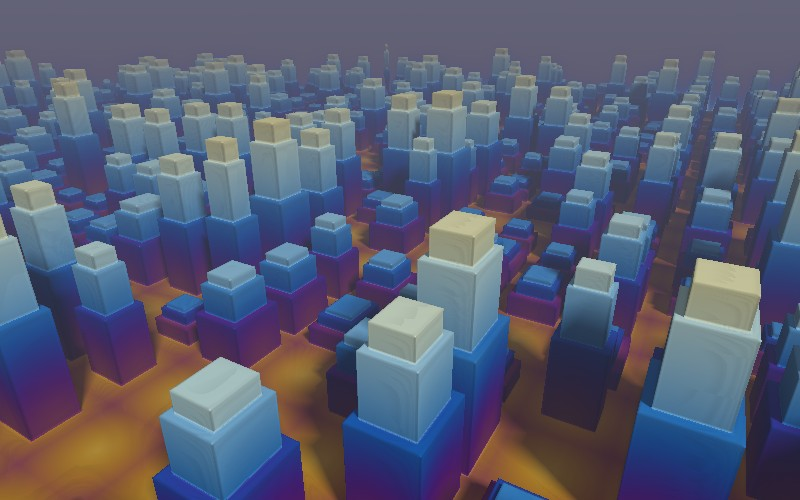
\includegraphics[width=0.88\textwidth]{img/skyline.jpg}
\caption{Skyline, default parameters (3 iterations).}\end{figure}
\paragraph{Parameters (app defaults).} Iterations 3 (range 1--5); step factor 0.8; bounding size 2; \emph{unbounded} (no bounding sphere assumed).

{\footnotesize\begin{tabular}{@{}llrr@{}}\toprule Parameter & Key & Default & Range\\\midrule
Block size & \texttt{cell} & 1 & 0.3\,\dots\,3\\
Height & \texttt{height} & 1.8 & 0.1\,\dots\,6\\
Height variety & \texttt{vary} & 0.75 & 0\,\dots\,1\\
Density & \texttt{density} & 0.8 & 0\,\dots\,1\\
Tower width & \texttt{width} & 0.32 & 0.15\,\dots\,0.42\\
Setback & \texttt{setback} & 0.25 & 0\,\dots\,0.8\\
Seed & \texttt{seed} & 7 & 0\,\dots\,100\\
\bottomrule\end{tabular}}


% =====================================================================
\section{Machines}

\subsection{Turbine}
\emph{Procedural, not a fractal.} $S=$ iterations stages stacked along $y$ at heights $y_k=(k+\tfrac12)g$ with radius $r_k=R\,\tau^k$ ($g$ = gap, $\tau$ = taper). Blades per stage: $N$, sector $\varsigma=2\pi/N$. For stage $k$:
\begin{align}
a&=\atantwo(q_z,q_x)+\text{spin}\cdot(-1)^{k+1},\qquad\vv q=\vv p-(0,y_k,0)\quad(\text{alternate stages counter-rotate}),\\
a'&=a-\varsigma\lfloor a/\varsigma+\tfrac12\rfloor,\qquad\vv b=\big(\rho\cos a',\ q_y,\ \rho\sin a'\big),\ \rho=\norm{\vv q_{xz}},\\
\vv b_{yz}&\leftarrow\begin{pmatrix}\cos\varphi&\sin\varphi\\-\sin\varphi&\cos\varphi\end{pmatrix}\vv b_{yz}\quad(\text{blade pitch }\varphi),\\
d_{\text{blade}}&=\sdbox\!\Big(\vv b-\big(\tfrac12(r_k+h),0,0\big),\ \big(\tfrac12(r_k-h),\ 0.012+0.04r_k,\ \chi\,r_k\big)\Big),\\
d_{\text{ring}}&=\norm{(\rho-r_k-0.03,\ q_y)}-0.025r_k,\qquad d_{\text{stage}}=0.9\min(d_{\text{blade}},d_{\text{ring}}).
\end{align}
$h$ = shaft radius, $\chi$ = blade width. The shaft is $\max\big(\norm{\vv p_{xz}}-h,\ \abs{p_y-\tfrac12\ell}-\tfrac12\ell-0.15\big)$ with $\ell=gS$. The result is the minimum of shaft and all stages.
\begin{figure}[H]\centering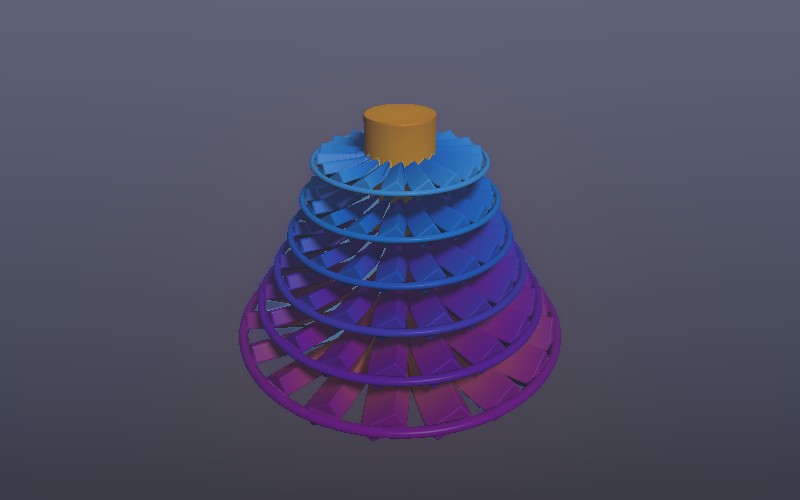
\includegraphics[width=0.88\textwidth]{img/turbine.jpg}
\caption{Turbine, default parameters (6 iterations).}\end{figure}
\paragraph{Parameters (app defaults).} Iterations 6 (range 1--12); step factor 0.7; bounding size 1.6.

{\footnotesize\begin{tabular}{@{}llrr@{}}\toprule Parameter & Key & Default & Range\\\midrule
Blades & \texttt{blades} & 18 & 2\,\dots\,40\\
Radius & \texttt{radius} & 1 & 0.3\,\dots\,2\\
Taper & \texttt{taper} & 0.86 & 0.5\,\dots\,1\\
Stage gap & \texttt{gap} & 0.22 & 0.05\,\dots\,0.6\\
Blade pitch & \texttt{pitch} & 35$^\circ$ & 0\,\dots\,80\\
Blade width & \texttt{chord} & 0.11 & 0.02\,\dots\,0.4\\
Shaft & \texttt{hub} & 0.2 & 0.02\,\dots\,0.6\\
Spin & \texttt{spin} & 0$^\circ$ & $-$180\,\dots\,180\\
\bottomrule\end{tabular}}


\subsection{Greeble hull}
Folded panels: every generation adds a plate, so plates carry plates. For each iteration (plate thickness $t$, seam depth $\epsilon$):
\begin{align}
\vv z&\leftarrow\Rot_A\,\mathrm{fold}_3(\abs{\vv z})\quad(\text{swap }xy,\ yz,\ xy\ \text{to sort}),\\
\vv q&=\vv z-(0,1-t,0),\qquad\vv g=\abs{\fract(2\vv q_{xz})-\tfrac12},\\
d_{\text{plate}}&=\sdbox(\vv q,(1,t,1))+\epsilon\,\mathrm{smoothstep}\!\big(0.06,0,\min(g_x,g_z)\big),\\
d&\leftarrow\min(d,\ d_{\text{plate}}/\mathrm{dr}),\qquad\vv z\leftarrow S_{s,\vv o}(\vv z),\quad\mathrm{dr}\leftarrow s\,\mathrm{dr}.
\end{align}
\begin{figure}[H]\centering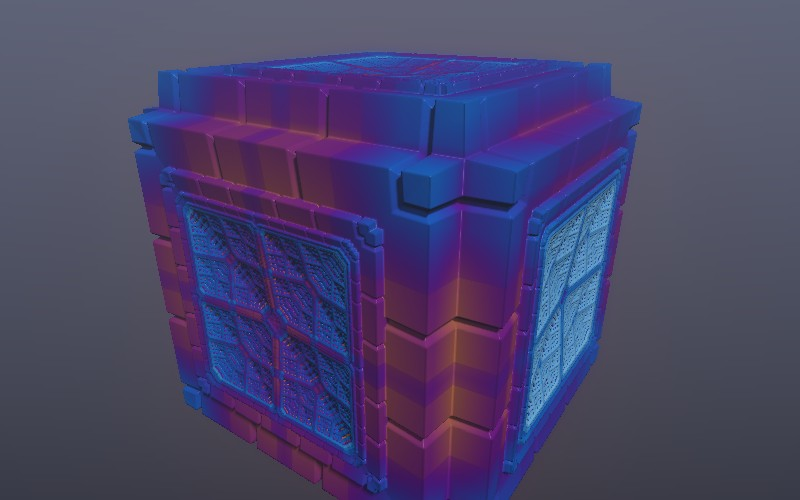
\includegraphics[width=0.88\textwidth]{img/greeble.jpg}
\caption{Greeble hull, default parameters (6 iterations).}\end{figure}
\paragraph{Parameters (app defaults).} Iterations 6 (range 1--12); step factor 0.8; bounding size 1.8.

{\footnotesize\begin{tabular}{@{}llrr@{}}\toprule Parameter & Key & Default & Range\\\midrule
Scale & \texttt{scale} & 2.3 & 1.5\,\dots\,3.5\\
Offset X & \texttt{offX} & 1 & 0\,\dots\,2\\
Offset Y & \texttt{offY} & 0.7 & 0\,\dots\,2\\
Offset Z & \texttt{offZ} & 0.45 & 0\,\dots\,2\\
Plate thickness & \texttt{plate} & 0.22 & 0.05\,\dots\,0.8\\
Panel seams & \texttt{inset} & 0.03 & 0\,\dots\,0.1\\
Rotation X & \texttt{rotX} & 0$^\circ$ & $-$180\,\dots\,180\\
Rotation Y & \texttt{rotY} & 0$^\circ$ & $-$180\,\dots\,180\\
Rotation Z & \texttt{rotZ} & 6$^\circ$ & $-$180\,\dots\,180\\
\bottomrule\end{tabular}}


\subsection{Pipeworks}
Each generation runs a pipe along $x$ from the centre, with a flange at its far end, and the symmetric fold maps the other axes onto it. Pipe radius $\rho_p$, joint radius $j$, $L=1$:
\begin{align}
\vv z&\leftarrow\Rot_A\sortd(\abs{\vv z}),\qquad d_{\text{pipe}}=\max\!\big(\norm{\vv z_{yz}}-\rho_p,\ z_x-L\big),\\
\vv f&=\big(\norm{\vv z_{yz}}-j,\ \abs{z_x-L}-0.35\,j\big),\qquad d_{\text{fl}}=\min(\max(f_x,f_y),0)+\norm{\max(\vv f,0)},\\
d&\leftarrow\min\!\big(d,\ \min(d_{\text{pipe}},d_{\text{fl}})/\mathrm{dr}\big),\qquad\vv z\leftarrow S_{s,\vv o}(\vv z),\ \ \mathrm{dr}\leftarrow s\,\mathrm{dr}.
\end{align}
With $s=3$ and $o_x=1.5$ each smaller cross sits exactly on a pipe end.
\begin{figure}[H]\centering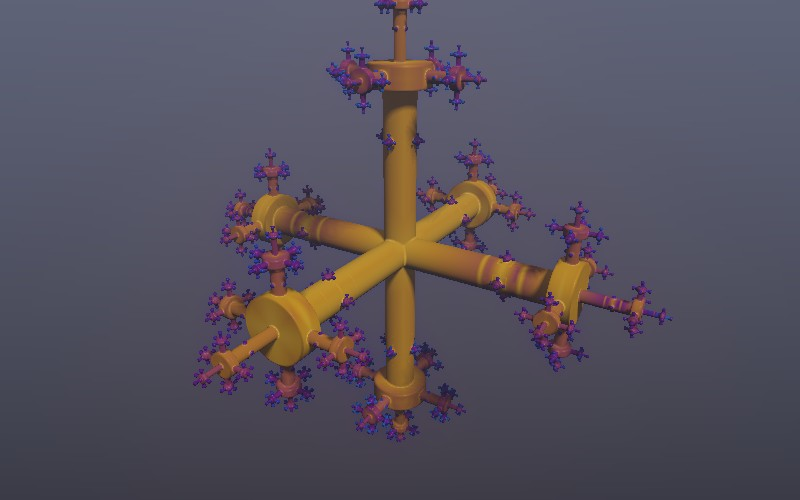
\includegraphics[width=0.88\textwidth]{img/pipeworks.jpg}
\caption{Pipeworks, default parameters (4 iterations).}\end{figure}
\paragraph{Parameters (app defaults).} Iterations 4 (range 1--10); step factor 0.8; bounding size 1.8.

{\footnotesize\begin{tabular}{@{}llrr@{}}\toprule Parameter & Key & Default & Range\\\midrule
Scale & \texttt{scale} & 3 & 1.5\,\dots\,4\\
Offset X & \texttt{offX} & 1.5 & 0\,\dots\,2\\
Offset Y & \texttt{offY} & 0 & 0\,\dots\,2\\
Offset Z & \texttt{offZ} & 0 & 0\,\dots\,2\\
Pipe radius & \texttt{pipe} & 0.09 & 0.02\,\dots\,0.5\\
Joint size & \texttt{joint} & 0.17 & 0\,\dots\,1\\
Rotation X & \texttt{rotX} & 0$^\circ$ & $-$180\,\dots\,180\\
Rotation Y & \texttt{rotY} & 0$^\circ$ & $-$180\,\dots\,180\\
Rotation Z & \texttt{rotZ} & 0$^\circ$ & $-$180\,\dots\,180\\
\bottomrule\end{tabular}}


\subsection{Piston field}
An endless periodic deck of telescoping pistons. Cell size $c$, block $\vv i=\lfloor p_{xz}/c\rfloor$, local coordinates $\vv q$ relative to the cell centre, rod radius $r_0=\text{radius}\cdot c$. Phase and rod height:
\begin{align}
\mathrm{ph}&=2\pi\big(\phi+\omega\cdot0.11\,(0.7\,i_x+1.3\,i_z)\big),\qquad H=\max\!\big(h_0+\Delta(\tfrac12+\tfrac12\sin\mathrm{ph}),\,0.02\big),
\end{align}
($\phi$ = phase, $\omega$ = wave, $h_0$ = rest height, $\Delta$ = stroke). With the cylinder distance
$\mathrm{cyl}(\vv q;r,y_0,y_1)=\min(\max(e_x,e_y),0)+\norm{\max(\vv e,0)}$, $\vv e=(\norm{\vv q_{xz}}-r,\ \abs{q_y-\tfrac12(y_0+y_1)}-\tfrac12(y_1-y_0))$, the pistons are $S$ stacked stages
\begin{equation}
\mathrm{cyl}\big(\vv q;\ r_0(1-0.18k),\ kH/S-0.01,\ (k+1)H/S\big),\ k=0..S-1,
\end{equation}
plus a cap $\mathrm{cyl}(\vv q;\,r_0(0.9+0.9\kappa),\,H,\,H+0.12c(\tfrac12+\kappa))$ and a deck with a collar round each rod; the result is clipped to the cell boundary.
\begin{figure}[H]\centering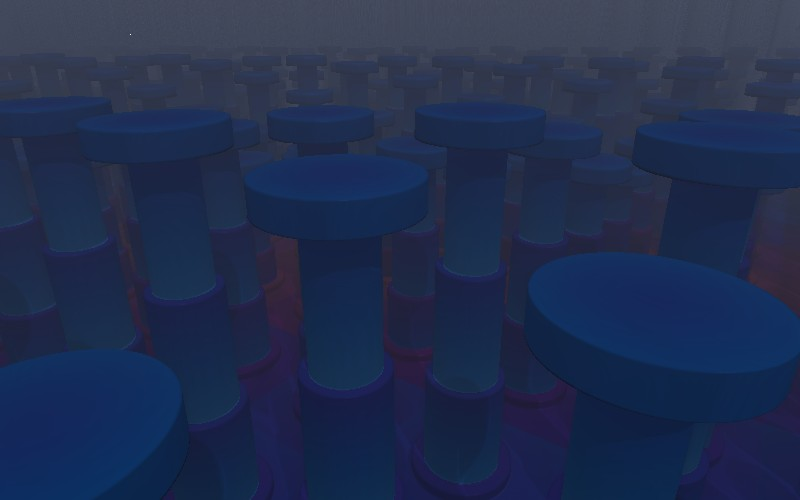
\includegraphics[width=0.88\textwidth]{img/pistons.jpg}
\caption{Piston field, default parameters (3 iterations).}\end{figure}
\paragraph{Parameters (app defaults).} Iterations 3 (range 1--4); step factor 0.7; bounding size 2; \emph{unbounded} (no bounding sphere assumed).

{\footnotesize\begin{tabular}{@{}llrr@{}}\toprule Parameter & Key & Default & Range\\\midrule
Spacing & \texttt{cell} & 0.7 & 0.3\,\dots\,2\\
Radius & \texttt{radius} & 0.22 & 0.05\,\dots\,0.48\\
Rest height & \texttt{base} & 0.8 & 0\,\dots\,3\\
Stroke & \texttt{stroke} & 0.6 & 0\,\dots\,2\\
Phase & \texttt{phase} & 0 & 0\,\dots\,1\\
Wave & \texttt{wave} & 1 & 0\,\dots\,3\\
Cap & \texttt{cap} & 0.5 & 0\,\dots\,1\\
\bottomrule\end{tabular}}


\subsection{Clockwork}
Gears carrying rings of smaller, \emph{meshing} gears. Generation $i$ has $n_i=\max(\mathrm{round}(T/s^i),6)$ teeth, direction $\delta_i=(-1)^i$ and speed $v_i=s^i$. With $a=\atantwo(z_z,z_x)+\text{spin}\,\delta_iv_i$, $r=\norm{\vv z_{xz}}$, $R=1$ (the frame is rescaled each step), tooth depth $t$, thickness $\vartheta$:
\begin{align}
\text{rim}&=r-\Big(R-t+t\big(\tfrac12+\tfrac12\clamp(2.5\cos(n_ia),-1,1)\big)\Big),\\
\text{hole}&=\max\!\Big(0.3R-r,\ r-(0.3+0.42\,\text{win})R,\ 0.09R-\Delta a\,r\Big),\\
\Delta a&=\Big|\big((a+\tfrac{\varsigma_5}2)\bmod\varsigma_5\big)-\tfrac{\varsigma_5}2\Big|,\quad \varsigma_5=\tfrac{2\pi}5\quad(\text{five spokes}),\\
g&=\max\!\Big(0.6\max\big(\max(\text{rim},-\text{hole}),\ 0.05R-r\big),\ \abs{z_y}-\vartheta\Big),\\
g&\leftarrow\min\!\big(g,\ \max(r-0.09R,\ \abs{z_y}-1.8\vartheta)\big)\quad(\text{axle}),
\end{align}
and $d\leftarrow\min(d,g/\mathrm{dr})$. Children: fold the azimuth into one of $m$ sectors ($\varsigma=2\pi/m$), then
\begin{equation}
\vv z\leftarrow s\,\Rot_A\big(\vv z-(R+R/s-t,\ \text{lift},\ 0)\big),\qquad\mathrm{dr}\leftarrow s\,\mathrm{dr}.
\end{equation}
Spinning the big gear turns every generation at its gear ratio.
\begin{figure}[H]\centering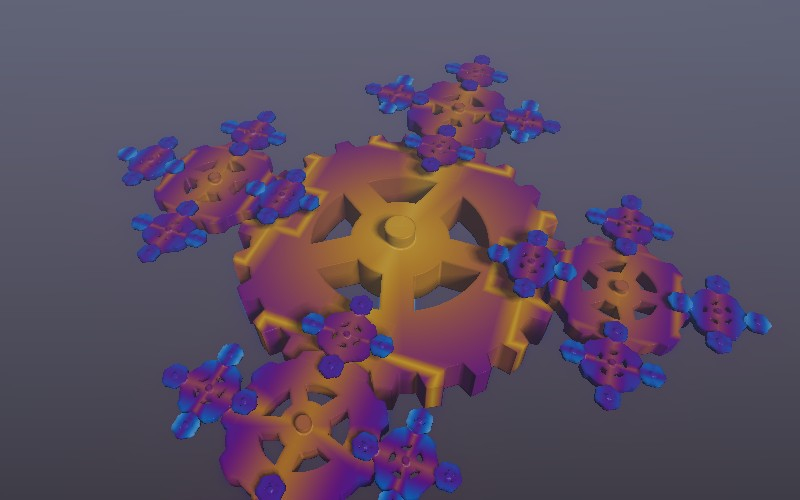
\includegraphics[width=0.88\textwidth]{img/clockwork.jpg}
\caption{Clockwork, default parameters (4 iterations).}\end{figure}
\paragraph{Parameters (app defaults).} Iterations 4 (range 1--6); step factor 0.6; bounding size 1.8.

{\footnotesize\begin{tabular}{@{}llrr@{}}\toprule Parameter & Key & Default & Range\\\midrule
Teeth & \texttt{teeth} & 24 & 6\,\dots\,48\\
Ratio & \texttt{ratio} & 2.6 & 1.8\,\dots\,4\\
Gears per ring & \texttt{around} & 4 & 2\,\dots\,8\\
Tooth depth & \texttt{tooth} & 0.09 & 0.02\,\dots\,0.25\\
Thickness & \texttt{thick} & 0.12 & 0.03\,\dots\,0.5\\
Stack & \texttt{lift} & 0.14 & $-$0.5\,\dots\,0.5\\
Windows & \texttt{windows} & 0.6 & 0\,\dots\,1\\
Spin & \texttt{spin} & 0$^\circ$ & $-$180\,\dots\,180\\
Tilt X & \texttt{rotX} & 0$^\circ$ & $-$180\,\dots\,180\\
Tilt Y & \texttt{rotY} & 0$^\circ$ & $-$180\,\dots\,180\\
Tilt Z & \texttt{rotZ} & 0$^\circ$ & $-$180\,\dots\,180\\
\bottomrule\end{tabular}}


\subsection{Truss}
Girder frames with diagonal braces, each holding smaller frames at its corners. With half-extents $\vv b=(L,\tfrac12,\tfrac12)$ ($L$ = stretch) and beam half-thickness $e$ the frame distance (box-frame SDF) is
\begin{align}
\vv p'&=\abs{\vv z}-\vv b,\quad\vv q'=\abs{\vv p'+e}-e,\\
d_{\text{frame}}&=\min\Big(\,g(p'_x,q'_y,q'_z),\ g(q'_x,p'_y,q'_z),\ g(q'_x,q'_y,p'_z)\Big),\quad g(\vv u)=\norm{\max(\vv u,0)}+\min(\max(u_x,u_y,u_z),0),
\end{align}
plus three diagonal rods (capsule distance, radius $0.7\,e\,\beta$) in the $\abs{\vv z}$ octant when the brace amount $\beta>0$. Per iteration:
\begin{equation}
d\leftarrow\min\big(d,\ d_{\text{frame}}/\mathrm{dr}\big);\quad\vv z\leftarrow\abs{\vv z},\ \text{sort }y\ge z;\quad\vv z\leftarrow s\,\Rot_A\vv z-\vv o\,(s-1)\odot(2L,1,1);\quad\mathrm{dr}\leftarrow s\,\mathrm{dr}.
\end{equation}
\begin{figure}[H]\centering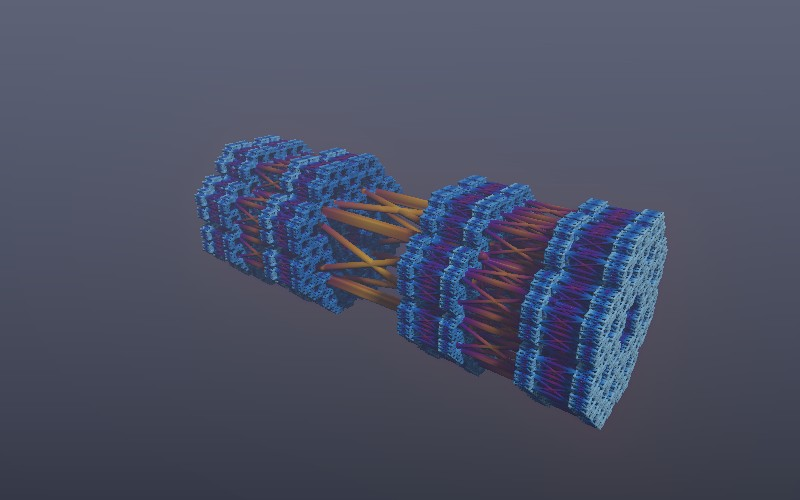
\includegraphics[width=0.88\textwidth]{img/truss.jpg}
\caption{Truss, default parameters (4 iterations).}\end{figure}
\paragraph{Parameters (app defaults).} Iterations 4 (range 1--7); step factor 0.8; bounding size 1.6.

{\footnotesize\begin{tabular}{@{}llrr@{}}\toprule Parameter & Key & Default & Range\\\midrule
Scale & \texttt{scale} & 2.6 & 1.8\,\dots\,4\\
Offset X & \texttt{offX} & 1 & 0\,\dots\,2\\
Offset Y & \texttt{offY} & 1 & 0\,\dots\,2\\
Offset Z & \texttt{offZ} & 0.4 & 0\,\dots\,2\\
Beam & \texttt{beam} & 0.05 & 0.01\,\dots\,0.2\\
Braces & \texttt{brace} & 1 & 0\,\dots\,1\\
Stretch & \texttt{stretch} & 1.4 & 0.4\,\dots\,3\\
Rotation X & \texttt{rotX} & 0$^\circ$ & $-$180\,\dots\,180\\
Rotation Y & \texttt{rotY} & 0$^\circ$ & $-$180\,\dots\,180\\
Rotation Z & \texttt{rotZ} & 0$^\circ$ & $-$180\,\dots\,180\\
\bottomrule\end{tabular}}


\subsection{Reactor}
Finned rings on spokes, each carrying smaller rings tilted on their own axes. Ring of radius 1 with rectangular section (half-width $w$, half-depth $\mathrm{dp}$); $a=\atantwo(z_z,z_x)+\text{spin}$, $r=\norm{\vv z_{xz}}$:
\begin{align}
\vv q&=\abs{(r-1,\ z_y)}-(w,\mathrm{dp}),\qquad d_{\text{ring}}=\norm{\max(\vv q,0)}+\min(\max(q_x,q_y),0),\\
d_{\text{fin}}&=\max\!\Big(\mathrm{rect}\big(\abs{(r-1,z_y)}-(1.8w,\,0.85\,\mathrm{dp})\big),\ \Delta_F\,r-0.012\Big),\\
&\qquad F\text{ fins; }\Delta_F=\text{angular distance to the nearest fin},\\
d_{\text{ring}}&\leftarrow\min(d_{\text{ring}},\ 0.8\,d_{\text{fin}}),
\end{align}
and, for $S>0$ spokes, a spoke capsule and a hub $\norm{(r,z_y)}-1.4w$ are added with $\min$. Children: fold the azimuth into one of $m$ sectors, move to the ring's rim ($z_x\leftarrow z_x-1$), tilt by $\varphi$ in the $(y,z)$ plane and scale:
\begin{equation}
\vv z_{yz}\leftarrow\begin{pmatrix}\cos\varphi&\sin\varphi\\-\sin\varphi&\cos\varphi\end{pmatrix}\vv z_{yz},\quad\vv z\leftarrow s\vv z,\quad\mathrm{dr}\leftarrow s\,\mathrm{dr}.
\end{equation}
\begin{figure}[H]\centering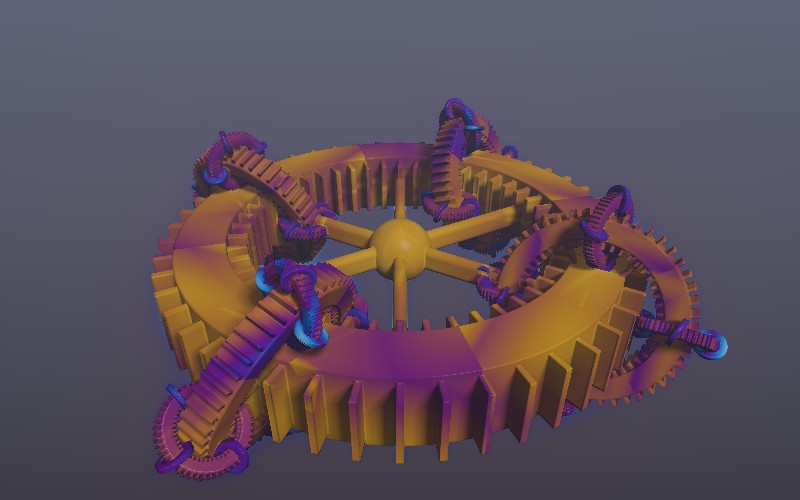
\includegraphics[width=0.88\textwidth]{img/reactor.jpg}
\caption{Reactor, default parameters (4 iterations).}\end{figure}
\paragraph{Parameters (app defaults).} Iterations 4 (range 1--6); step factor 0.7; bounding size 1.6.

{\footnotesize\begin{tabular}{@{}llrr@{}}\toprule Parameter & Key & Default & Range\\\midrule
Ratio & \texttt{ratio} & 2.7 & 1.8\,\dots\,4\\
Rings per ring & \texttt{around} & 4 & 2\,\dots\,8\\
Spokes & \texttt{spokes} & 6 & 0\,\dots\,12\\
Fins & \texttt{fins} & 48 & 0\,\dots\,96\\
Ring width & \texttt{width} & 0.12 & 0.03\,\dots\,0.4\\
Ring depth & \texttt{depth} & 0.18 & 0.02\,\dots\,0.5\\
Tilt & \texttt{tilt} & 70$^\circ$ & 0\,\dots\,90\\
Spin & \texttt{spin} & 0$^\circ$ & $-$180\,\dots\,180\\
\bottomrule\end{tabular}}


% =====================================================================
\section{Landscapes (heightfields)}
These are not volumetric fractals: each defines a height $h(x,z)$ and returns a scaled vertical distance $\DE=\lambda\,(y-h)$, with a safety factor $\lambda<1$ because the slope can exceed one.

\paragraph{Value noise.} $\mathrm{hash}(\vv v)$ as in Skyline (constants $234.34,435.345,34.23$ here); with $\vv i=\lfloor\vv q\rfloor$, $\vv f=\fract(\vv q)$, $\vv u=\vv f^2(3-2\vv f)$:
\begin{equation}n(\vv q)=\mathrm{lerp}\big(\mathrm{lerp}(h_{00},h_{10},u_x),\ \mathrm{lerp}(h_{01},h_{11},u_x),\ u_y\big).\end{equation}
The octave map is $\vv q\leftarrow M\vv q$ with $M=\begin{pmatrix}1.6&-1.2\\1.2&1.6\end{pmatrix}$ (a rotation by $36.9^\circ$ and scaling by 2).

\subsection{Folded terrain}
Ridged fractional Brownian motion with domain warping. $\vv q_0=f\,\vv p_{xz}+13.1\cdot\text{seed}$, ridge amount $\rho\in[0,1]$, roughness (gain) $G$, warp $W$:
\begin{align}
n_k&=(1-\rho)\,n(\vv q_k)+\rho\,\big(1-\abs{2n(\vv q_k)-1}\big),\qquad\Sigma_k=\Sigma_{k-1}+a_k n_k,\ \ a_k=G^k,\\
\vv q_{k+1}&=M\vv q_k+W\,(\Sigma_k,\ -\Sigma_k),\qquad h_n=\Sigma\Big/\sum a_k,\\
h&=\max\!\big(H\,(h_n-0.45),\ \text{sea}\big),\qquad\DE=0.55\,(p_y-h).
\end{align}
\begin{figure}[H]\centering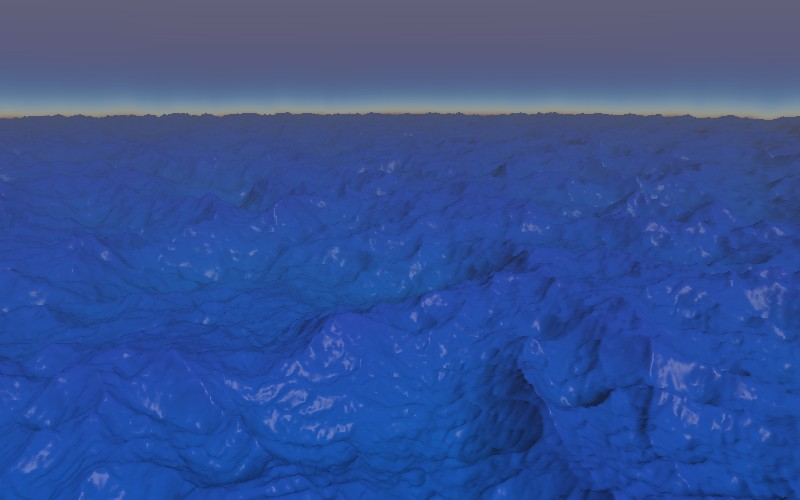
\includegraphics[width=0.88\textwidth]{img/terrain.jpg}
\caption{Folded terrain, default parameters (7 iterations).}\end{figure}
\paragraph{Parameters (app defaults).} Iterations 7 (range 2--10); step factor 0.45; bounding size 3; \emph{unbounded} (no bounding sphere assumed).

{\footnotesize\begin{tabular}{@{}llrr@{}}\toprule Parameter & Key & Default & Range\\\midrule
Feature size & \texttt{freq} & 0.6 & 0.1\,\dots\,3\\
Height & \texttt{height} & 1.4 & 0\,\dots\,4\\
Ridge & \texttt{ridge} & 0.7 & 0\,\dots\,1\\
Roughness & \texttt{gain} & 0.48 & 0.25\,\dots\,0.7\\
Warp & \texttt{warp} & 0.35 & 0\,\dots\,1.5\\
Sea level & \texttt{sea} & $-$0.35 & $-$1\,\dots\,1\\
Seed & \texttt{seed} & 3 & 0\,\dots\,100\\
\bottomrule\end{tabular}}


\subsection{Kali coral plain}
Ground grown from Kali's abs-inversion set, tiled by mirroring so it repeats without seams:
\begin{align}
\vv q_0&=1.2\,\Big|\,2\,\fract\!\big(\tfrac f4\,\vv p_{xz}+\tfrac12\big)-1\,\Big|,\qquad\vv q_{k+1}=\frac{\abs{\vv q_k}}{\max(\norm{\vv q_k}^2,10^{-3})}-\vv c,\ \ \vv c=(c_x,c_y),\\
\mathrm{acc}&=\sum_k\exp\!\big(-\gamma\,\big|\norm{\vv q_k}-\norm{\vv q_{k-1}}\big|\big),\qquad h_n=\clamp(\mathrm{acc}/N,0,1),\\
h&=\max(H\,h_n,\ \text{floor}),\qquad\DE=0.4\,(p_y-h).
\end{align}
$\gamma$ = \emph{Contrast}.
\begin{figure}[H]\centering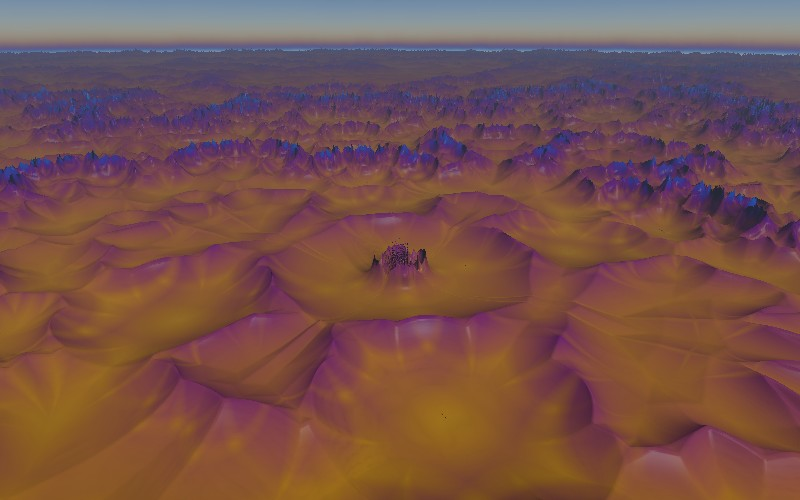
\includegraphics[width=0.88\textwidth]{img/kaliPlain.jpg}
\caption{Kali coral plain, default parameters (9 iterations).}\end{figure}
\paragraph{Parameters (app defaults).} Iterations 9 (range 3--20); step factor 0.35; bounding size 3; \emph{unbounded} (no bounding sphere assumed).

{\footnotesize\begin{tabular}{@{}llrr@{}}\toprule Parameter & Key & Default & Range\\\midrule
Feature size & \texttt{freq} & 0.12 & 0.02\,\dots\,2\\
Height & \texttt{height} & 0.7 & 0\,\dots\,3\\
C x & \texttt{cx} & 0.58 & 0\,\dots\,1.5\\
C y & \texttt{cy} & 0.73 & 0\,\dots\,1.5\\
Contrast & \texttt{focus} & 1.5 & 0.5\,\dots\,8\\
Floor & \texttt{floor} & $-$0.2 & $-$1\,\dots\,1\\
\bottomrule\end{tabular}}


\subsection{Eroded ridges}
Noise whose small detail fades on steep slopes, as erosion leaves it. Uses value noise \emph{with analytic derivatives} $(n,\ \partial_xn,\ \partial_zn)$. With $\vv D_k=\sum_{j\le k}\nabla n(\vv q_j)$ the accumulated gradient, erosion $\eta$, gain $G$:
\begin{align}
a&=\sum_k b_k\,\frac{n(\vv q_k)}{1+\eta\,\norm{\vv D_k}^2},\qquad b_k=G^k,\qquad h_n=a\Big/\sum_k b_k,\\
h_n'&=h_n-0.6\,\kappa\,\mathrm{smoothstep}(0.35,\ 0.15,\ h_n)\quad(\text{canyon amount }\kappa),\\
h&=H\,(h_n'-0.3),\qquad\DE=0.5\,(p_y-h).
\end{align}
\begin{figure}[H]\centering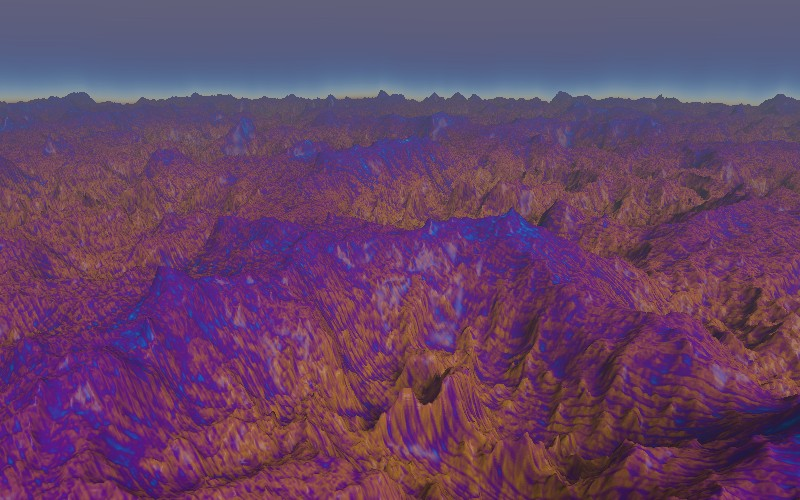
\includegraphics[width=0.88\textwidth]{img/ridges.jpg}
\caption{Eroded ridges, default parameters (8 iterations).}\end{figure}
\paragraph{Parameters (app defaults).} Iterations 8 (range 2--10); step factor 0.45; bounding size 3; \emph{unbounded} (no bounding sphere assumed).

{\footnotesize\begin{tabular}{@{}llrr@{}}\toprule Parameter & Key & Default & Range\\\midrule
Feature size & \texttt{freq} & 0.45 & 0.1\,\dots\,3\\
Height & \texttt{height} & 1.8 & 0\,\dots\,4\\
Erosion & \texttt{erosion} & 1.2 & 0\,\dots\,3\\
Roughness & \texttt{gain} & 0.5 & 0.25\,\dots\,0.7\\
Canyon & \texttt{canyon} & 0.3 & 0\,\dots\,1\\
Seed & \texttt{seed} & 11 & 0\,\dots\,100\\
\bottomrule\end{tabular}}


% =====================================================================
\appendix
\section{Quick reference: which equation is which}
\begin{center}\footnotesize
\begin{tabular}{@{}p{2.3cm}p{6.3cm}p{5.2cm}@{}}\toprule
Family & Formulas & Distance estimate\\\midrule
Escape-time & Mandelbulb, Quaternion Julia, Folded bulb hybrid & $\tfrac12 r\ln r/\mathrm{dr}$ (potential)\\
Box/sphere fold & Mandelbox, Amazing Box, Vaulted box, Amazing Surf & $\norm{\vv z}/\abs{\mathrm{dr}}$\\
Abs-inversion & KaliBox, Pseudo-Kleinian, Apollonian & scale-corrected\\
KIFS & Menger, Sierpinski, Octahedral, Kaleidoscopic, Icosahedral & $(\norm{\vv z}-1)/s^N$ or $\sdbox/s^N$\\
Hyperbolic & Hyperbolic honeycomb & $d/\mathrm{sc}$ in Poincar\'e ball\\
Branching & Tree, Dendrite, Nerve cell, Root, Mycelium, Coral & $\min_k \mathrm{cap}_k/\mathrm{dr}_k$\\
Procedural/IFS & Ziggurat, Skyline, Turbine, Greeble, Pipeworks, Pistons, Clockwork, Truss, Reactor & $\min_k(\text{primitive})/\mathrm{dr}$\\
Heightfield & Folded terrain, Kali coral plain, Eroded ridges & $\lambda(y-h)$\\
\bottomrule\end{tabular}
\end{center}

\end{document}
